\documentclass[12pt]{caltech_thesis}
\usepackage[hyphens]{url}
\usepackage{lipsum}
\usepackage{graphicx}
\usepackage{todonotes}
\usepackage[utf8]{inputenc}
\usepackage[T1]{fontenc}
\usepackage{mathpazo}
\usepackage[numbers,sort&compress]{natbib}
\usepackage{csquotes}
\usepackage{bibunits}
\usepackage{enumitem}
\usepackage{amsmath}
\usepackage{longtable}
\usepackage{xcolor} 
\usepackage{indentfirst} 
\usepackage{upgreek} % for non-italic greek letters (units)
\usepackage[outputdir=../]{minted} % for code highlighting
% custom output dir following this solution: https://tex.stackexchange.com/questions/531738/minted-environment-not-working-in-overleaf

\definecolor{CaltechOrange}{HTML}{FF6C0C}
\definecolor{midnightblue}{HTML}{191970}
\definecolor{darkred}{HTML}{BA1A1A}
\usepackage[hidelinks=true,
            colorlinks=true, 
            linkcolor=black,
            urlcolor=CaltechOrange, 
            linkbordercolor=white,
            backref=false,
            pagebackref=false,
            hyperindex=false,
            breaklinks=true,
            bookmarks=false,
            bookmarksopen=false,
            ]{hyperref}
\usepackage[
            backend=biber,natbib,
            % IMPORTANT: load a style suitable for your discipline
            style=ieee
        ]{biblatex}


% added to conform with this issue: https://github.com/jgm/pandoc/issues/4384
% with this, figure width can be changed with {width: 70%}
\makeatletter
\def\maxwidth{\ifdim\Gin@nat@width>\linewidth\linewidth\else\Gin@nat@width\fi}
\def\maxheight{\ifdim\Gin@nat@height>\textheight\textheight\else\Gin@nat@height\fi}
\makeatother
% Scale images if necessary, so that they will not overflow the page
% margins by default, and it is still possible to overwrite the defaults
% using explicit options in \includegraphics[width, height, ...]{}
\setkeys{Gin}{width=\maxwidth,height=\maxheight,keepaspectratio}

\hypersetup{
  colorlinks = true,
  linkcolor = black
}

\makeatletter
\let\@mycite\@cite
\def\@cite#1#2{{\hypersetup{linkcolor=black!60!black}[{#1\if@tempswa , #2\fi}]}}
\makeatother
            
\addbibresource{references.bib}
\defaultbibliographystyle{plainnat}
\renewcommand{\bibsection}{\section*{\refname}}
\usepackage{memhfixc}
\linespread{1.5}


\begin{document}

\title{Towards Precise Quantum Measurements with Superconducting
Nanowire Single Photon Detectors}
\author{Andrew Sterling Mueller}
\degreeaward{Doctor of Philosophy in Applied Physics}                 
\university{California Institute of Technology}    
\address{Pasadena, California}                     
\unilogo{caltech.png}                                 
\copyyear{2024}  
\defenddate{November 2023}   
       
\orcid{0000-0002-6598-9732}



\rightsstatement{Some rights reserved. This thesis is distributed under
a Creative Commons Attribution License CC-BY 4.0. All software used in
the analysis and generation of figures is distributed under an MIT
license, and is available on a GitHub repository
\href{https://github.com/sansseriff/phd_thesis}{https://github.com/sansseriff/phd\textunderscore thesis}}

\maketitle[logo]

\begin{acknowledgements}   
    \input{frontmatter/acknowledgements.md}
\end{acknowledgements}

\begin{abstract}
  \input{frontmatter/abstract.md} 
\end{abstract}

\extrachapter{Published Content and Contributions}
\begin{publishedcontent}
\input{frontmatter/published.md}
\end{publishedcontent}

\tableofcontents
\listoffigures
\listoftables
\printnomenclature
\mainmatter

\hypertarget{low-dark-count-rate-detection}{%
\chapter{Low Dark Count Rate
Detection}\label{low-dark-count-rate-detection}}

~~~~~~~~~~~~~~~~~~~~~~~~~~~~~~~~~~~~~~~~~~~~~~~\includegraphics{chapter_01/figs_01/dark_counts.png}

\hypertarget{abstract}{%
\section{Abstract}\label{abstract}}

This is an overview of the dark count minimization section. More details
to come. H

This is a crazy number of bounces in your head.

And here's some more

\hypertarget{introduction}{%
\section{Introduction}\label{introduction}}

Time-resolved photon detection with low dark counts is a vital
technology in fields such as quantum information processing, classical
communication, quantum communication, and laser ranging. Increasingly,
research in these fields employs superconducting nanowire single photon
detectors (SNSPDs), which have been demonstrated with system detection
efficiency (\(\eta\)) of more than 90\% \autocite{Reddy2020}, timing
jitter (\(\Delta t\)) as low as 2.6 ps \autocite{Korzh2020} and
intrinsic dark count rates (\(D\)) in the milli- to micro-hertz range
\autocite{Hochberg2019}. However, quantum communication applications
require detection systems with performance optimized across all three
metrics simultaneously. The dimensionless figure of merit \(H\)
specifies this application-specific performance as
\(H = \frac{\eta}{(\Delta t D)}\) \autocite{Hadfield2009}.

Here, we focus on lowering the Dark Count Rate (DCR) of a telecom-band
SNSPD system by filtering thermal photons, without sacrificing
efficiency or jitter. We demonstrate a free-space coupled SNSPD with
sub-0.1 Hz DCR, 14 ps timing jitter, and 72\% total system detection
efficiency (SDE) by using a differential single-pixel SNSPD
\autocite{Colangelo2021} to image a single-mode fiber through an
optimized free-space filter stack.

The highest system detection efficiencies have been achieved using
self-aligned fiber coupling where dark counts can be reduced using
cryogenic fiber looping \autocite{Cohen2015} or spliced narrow-band
filters \autocite{Boaron2018secure}. But it is difficult to achieve
strong filtering without losses at the target wavelength. Low-loss,
high-rejection filters are typically available as free-space components,
so some of the highest reported H-values were achieved with cryogenic,
fiber to free-space to fiber coupling, but exhibit an SDE of only a few
percent \autocite{Shibata2015}. The filtering method presented here
takes advantage of commercially-available filters, achieves a high
free-space coupling efficiency using a cryogenic lens, and is compatible
with both fiber and free-space optical inputs.

In this work, a single mode fiber is imaged onto the detector using two
f = 18.75 mm lenses. One lens collimates light from an optical fiber
face outside the cryostat (Photon Spot), and the other focuses light
onto the detector inside \autocite{Bellei:16}. In the collimated region
between, the beam passes though a series of short-pass filters and one
band-pass filter mounted at 4 K (Fig. \ref{fig:setup}a). One of the
short-pass filters is angled to avoid ghosting effects. The 40 K
radiation shield and outer cryostat housing are fitted with
anti-reflection coated BK7 windows. The filters are spring loaded to
prevent cracking at low temperatures. To minimize effects of stray
light, the interior of the 4 K shield was painted with mid-IR absorbing
paint (Aeroglaze Z306) \autocite{Persky1999}, while gaps between filters
and the windows were covered with metal tape.

The system is based on 1-inch optics, although the f = 18.75 mm lenses
lead to a \(1/e^2\) intensity diameter of about 5 mm in the collimated
region. To reduce the larger-than-required numerical aperture of the
system, painted 8 mm apertures (Acktar Spectral Black) were added in the
collimated region. These are large enough to allow minor alignment
adjustments --- by translating the exterior collimating lens --- without
vignetting.

\hypertarget{fig:dcrmin_data}{%
\begin{figure}
\centering
\includegraphics{chapter_01/figs_01/DataFigure_6.pdf}
\caption[{Low Dark Count Rate Project Results.}]{\textbf{Low Dark Count
Rate Project Results} a) Simulated photon flux at various temperatures
with and without the 1550 nm bandpass filter (BP). b) Normalized photon
count rate (PCR) and jitter measurements c) DCR, and calculated figure
of merit \(H\) versus bias current for both fiber-coupled and free space
coupled configurations.}
\label{fig:dcrmin_data}
\end{figure}
}

We use four custom cryogenic short-pass filters, with pass-bands below
\(1.6 \ \mathrm{\upmu m}\) and \(1.9 \ \mathrm{\upmu m}\) (Andover
Corp.), both with transmission at 1550 nm of 98.8 ± 0.3\%. They reject
wavelengths shorter than \(3 \ \mathrm{\upmu m}\) through reflective
optical coatings, and attenuate longer wavelengths through material
absorption in the 12.7 mm-thick N-BK7 glass substrate. While the
bandpass filter (FWHM = 7 nm) was found to blue-shift by about 2 nm at
cryogenic temperatures, the passband was wide enough such that
significant attenuation was not observed at the original target
wavelength of 1550 nm. This filter is also sufficiently wide to avoid
Fourier-limited broadening of ultra-short laser pulses.

The filtering of the optical stack was modeled by assuming a black-body
emitter at 298 K and a field of view defined by the 18.75 mm focal
length of the cryogenic lens and the 8 mm diameter of the apertures. The
resulting spectrum was multiplied by the transmission of the filters
(Fig. \ref{fig:setup}b) and detector optical stack (Fig.
\ref{fig:setup}c). The model showed that two each of the
\(1.6 \ \mathrm{\upmu m}\) and \(1.9 \ \mathrm{\upmu m}\) short pass
filters were necessary to suppress mid-infrared light to where it was no
longer the dominant source of dark counts. With the inclusion of the
four shortpass filters, the dominant source of dark counts is the
spectral region near 1550 nm as shown in Fig. \ref{fig:false-color}a,
which also illustrates the effect of the bandpass filter. Also evident
in Fig. \ref{fig:false-color}a is the strong dependence of DCR on the
temperature of the final surface outside the cryostat emitting thermal
radiation. This motivated the exterior cooling apparatus shown at the
bottom of Fig. \ref{fig:setup}a. The bulkhead holding the fiber
connector is cooled to around -2\(^\circ\)C using a Peltier element and
liquid cooling block. This addition reduced the system DCR from 0.4 Hz
to below 0.1 Hz. While dark counts from multiple spatial modes are
present in this system --- modes that would not be present in a purely
fiber based approach --- the external cooling technique works to
minimize their effect.

This work used a low-jitter, differential SNSPD \cite{Colangelo2021},
with an active area of \(22 \times 15 \ \mathrm{\upmu m}\), formed by a
meander of 100 nm-wide and 5-nm-thick niobium nitride (NbN) nanowires on
a 500 nm pitch. A more conventional single-ended readout SNSPD of
similar area would also achieve low DCR in this coupling system, but
would likely achieve a lower performance metric \(H\) from
correspondingly higher jitter. The nanowire is embedded in an
efficiency-enhancing optical stack made of alternating layers of
TiO\(_2\) and SiO\(_2\) and a gold mirror layer. As shown in Fig.
\ref{fig:false-color}b and c, when fiber coupled (without any
fiber-based filtering methods applied), this detector achieved a
saturated SDE of \(84\% \pm 4.4 \%\) and a DCR of 20 Hz at a bias
current of \(16\ \mathrm{\upmu A}\).

~~~~~ As also shown in Fig. \ref{fig:false-color}b, the free-space
coupling system achieves up to \(72 \% \pm 3.7 \%\) SDE as measured from
the fiber outside the cryostat. The reduction in efficiency is likely
due to surface reflections in the free-space optics, and potential
misalignment in the optical baffles. The minimum DCR (Fig.
\ref{fig:false-color}c) at \(72 \%\) SDE is about 0.1 Hz, with a bias
current of 16 \(\mathrm{\upmu A}\). These metrics, with the jitter
measurements shown in Fig. \ref{fig:false-color}b, give a maximum H
value of \(5 \times 10^{11}\) (Fig. \ref{fig:false-color}c). Values as
high as \(1.8 \times 10^{12}\) have been reported before, but at 1.5\%
system detection efficiency \cite{Shibata2015}. Our system shows a low
DCR can be achieved without severe reduction of SDE or usable target
wavelength bandwidth. This is paramount for the future of terrestrial
and space-to-ground quantum communication, since it increases success
rate with finite statistics \cite{Boaron2018secure}. The same techniques
can be applied to emerging SNSPD applications at longer wavelengths,
such as laser ranging \cite{Taylor2019}, where fiber filtering is
impractical. Beyond single-mode applications, our work paves the way to
scalable, low-DCR, multi-mode coupling to SNSPD arrays
\cite{Wollman2019}.

\hypertarget{fig:custom_figure}{%
\begin{figure}
\centering
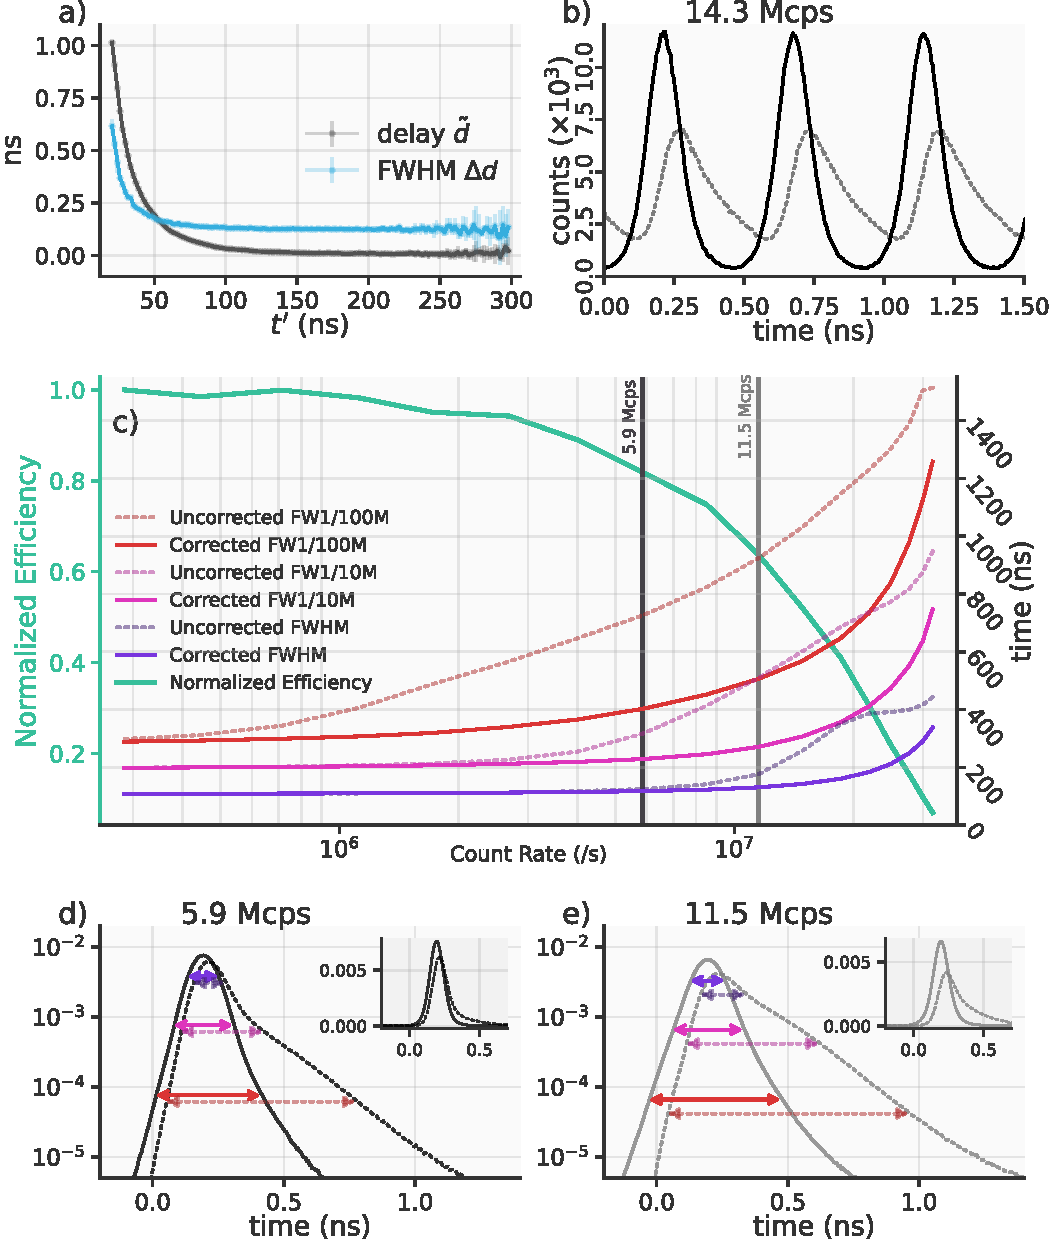
\includegraphics[width=0.7\textwidth,height=\textheight]{chapter_01/figs_01/Figure_Data_Sept_2022_light.pdf}
\caption[{A jitterate data figure.}]{\textbf{Figure Title.} And I think
the rest of this is the caption with (A), (B), and (C) callouts}
\label{fig:custom_figure}
\end{figure}
}

Finally, here's a png figure for testing

\hypertarget{fig:test_png_figure}{%
\begin{figure}
\centering
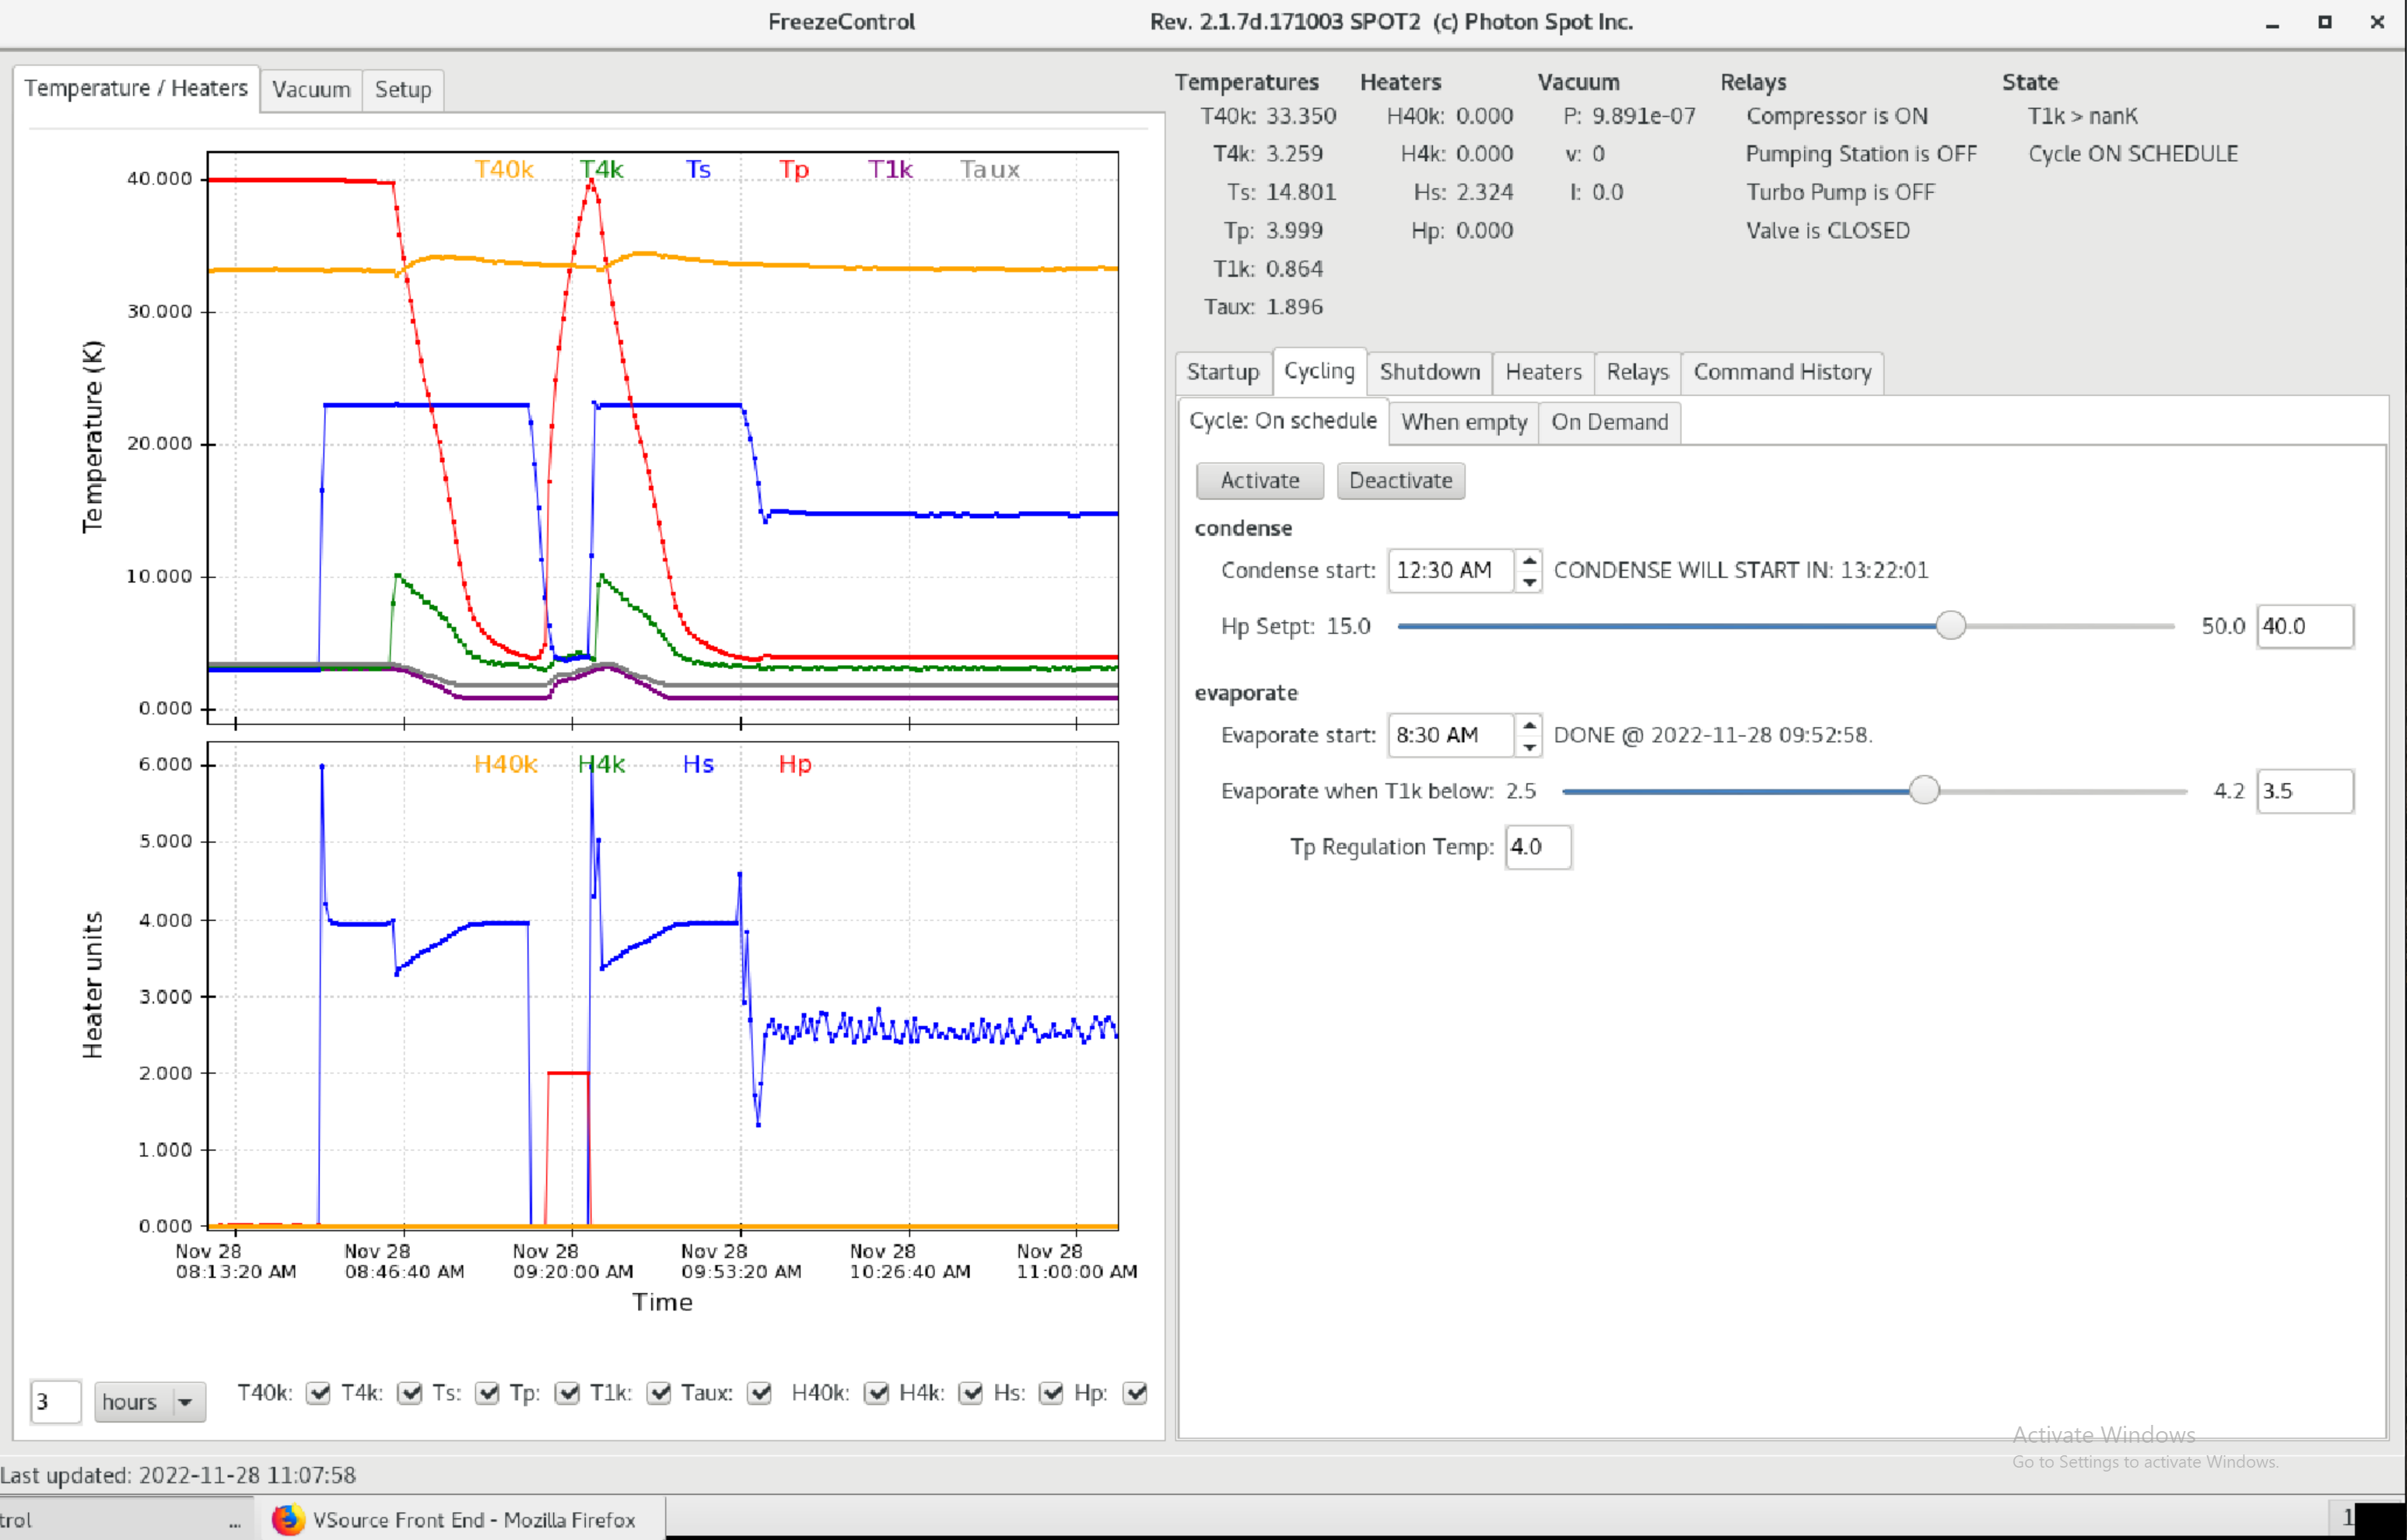
\includegraphics[width=0.7\textwidth,height=\textheight]{chapter_01/figs_01/fridge.png}
\caption[{A png figure.}]{\textbf{A test png figure.} And here is where
I'd put in more information about the png.}
\label{fig:test_png_figure}
\end{figure}
}

Remember there's a lot of optics stuff you got good at, like how to
focus a spot inside the fridge using only optics outside the fridge. How
you used the xyz stage on the fiber for that, and the xy or the mirror.
How you defocused the laser to see the detector when you were using the
narroband filter.

\hypertarget{high-rate-pulse-position-modulation}{%
\chapter{High Rate Pulse Position
Modulation}\label{high-rate-pulse-position-modulation}}

~~~~~~~~~~~~~~~~~~~~~~~~~~~~~~\includegraphics{chapter_02/figs_02/pnr_and_pulses.png}

\hypertarget{abstract-1}{%
\section{Abstract}\label{abstract-1}}

~~~~~ This study aimed to evaluate the feasibility of transmitting high
clock-rate pulse position modulated (PPM) data using a mode-locked laser
and receiving it with a low jitter superconducting nanowire
single-photon detector (SNSPD). The investigation was driven by recent
advancements in NbN SNSPDs, which have achieved a jitter as low as 50 ps
at the FW(1/100)M level, enabling the demonstration of PPM with 50 ps
slot widths and a 20 GHz clock. The aim was to increase the data rate by
a factor of 10, from 2 GHz to 20 GHz, in the next generation of the Deep
Space Optical Communication (DSOC) project.

During the course of this study, the focus shifted towards investigating
the impact of photon number resolution (PNR) on the low jitter detection
of optical pulses. PNR can have an unintended impact on the
demonstration of high-rate PPM, and therefore a thorough study of its
effects was deemed crucial. A novel PNR cancellation technique was
developed and applied to successfully demonstrate high-rate PPM. This
technique is considered essential for future low-jitter applications of
SNSPDs that exhibit photon-number effects.

\hypertarget{introduction-1}{%
\section{Introduction}\label{introduction-1}}

~~~~~ This study aimed to evaluate the feasibility of transmitting high
clock-rate pulse position modulated (PPM) data using a mode-locked laser
and receiving it with a low jitter superconducting nanowire
single-photon detector (SNSPD). The investigation was driven by recent
advancements in NbN SNSPDs, which have achieved a jitter as low as 50 ps
at the FW(1/100)M level, enabling the demonstration of PPM with 50 ps
slot widths and a 20 GHz clock. The aim was to increase the data rate by
a factor of 10, from 2 GHz to 20 GHz, in the next generation of the Deep
Space Optical Communication (DSOC) project.

During the course of this study, the focus shifted towards investigating
the impact of photon number resolution (PNR) on the low jitter detection
of optical pulses. PNR can have an unintended impact on the
demonstration of high-rate PPM, and therefore a thorough study of its
effects was deemed crucial. A novel PNR cancellation technique was
developed and applied to successfully demonstrate high-rate PPM. This
technique is considered essential for future low-jitter applications of
SNSPDs that exhibit photon-number effects.

\hypertarget{pulse-position-modulation-for-deep-space-communication}{%
\subsection{Pulse Position Modulation for Deep Space
Communication}\label{pulse-position-modulation-for-deep-space-communication}}

~~~~~ Deep Space Optical Communication has been a growing field of study
in recent years, as researchers look for ways to communicate with
spacecraft that are far away from Earth. In this article, we will focus
on the use of Pulse Position Modulation (PPM) for deep space optical
communication.

While other modulation techniques such as quadrature amplitude
modulation (QAM) have been used in the past, it has been shown that in
the photon-starved regime, PPM is the best approach for sending data.
This is because there is not enough light to measure the phase of the
signal.

PPM relies on sending one optical pulse carrying M bits of information
in one of \(2^M\) possible time slots. For M = 2, this corresponds to
sending an early pulse to represent a 0 bit and a late pulse to
represent a 1 bit.

The main challenge in deep space optical communication is the high loss
and distance that the link must traverse. This limits the communication
from the spacecraft, as it is limited by the power available on the
spacecraft. This means that the communication protocol is limited by the
number of bits that can be sent per unit of energy on the spacecraft,
also known as photon information efficiency or bits per photon.

For large M, PPM achieves high photon information efficiency, allowing
for the saving of power on the spacecraft and the sending of more
information with fewer photons. The existing deep space optical
communication project uses M up to \(2^8 = 256\), meaning that 8 bits of
data are carried in each optical pulse.

In this project, we aimed to demonstrate even higher photon information
efficiency by using M values up to 2048, or 11 bits of data per optical
pulse.

While the use of large M values increases photon information efficiency,
it also decreases the data rate of the system. This is because the
number of time bins needed per optical pulse scales exponentially with
the amount of data in each pulse. Therefore, for a given fixed clock
rate and time bin duration, the data rate decreases dramatically for
higher M values.

Using M values much larger than 11 is unlikely to be practical in future
deep space optical communication systems. However, the data rate of
these systems can be increased linearly by increasing the clock rate or
bin size of the experiment. This is possible with the use of low jitter
detection systems or low jitter superconducting nanowire single-photon
detectors (SNSPDs).

\hypertarget{development-of-a-modulation-source}{%
\subsection{Development of a modulation
source}\label{development-of-a-modulation-source}}

~~~~~ The communication signal on a spacecraft is generated by utilizing
a Continuous Wave (CW) seed laser that is carved by a fast intensity
modulator. The resulting low-power pulsed signal is then amplified by an
Erbium Doped Fiber Amplifier (EDFA) to increase its transmission power
to Earth. The majority of the power used by the spacecraft for
communication scales with the number of optical pulses due to the EDFA.

In our experiment, the 20 GHz repetition rate was limited by the jitter
of the Single-Photon Detectors (SNSPDs) that we intended to use. These
detectors have a Full Width at Half Maximum (FW(1/100)M) jitter of
approximately 50 ps. To ensure that the response function of the entire
experiment had jitter of around 50 ps FW(1/100)M, we needed to build a
Pulsed Phase Modulation (PPM) source with ultra-short optical pulses.

Carving a CW laser with our system would have introduced excessive
timing uncertainty due to the limited ability of even the fastest
lithium niobate intensity modulators to carve pulses with widths below
20 ps. The added jitter from modulated CW pulses, combined with the
jitter of the detectors, would have exceeded the 20 GHz/50 ps slot width
requirement.

Therefore, we chose to carve pulses from a mode-locked laser. This
approach allows for extremely short pulses in time, with the modulators
responsible for sufficiently reducing any surrounding unwanted pulses.
The temporal width of the modulator pulse response must be extremely
short and able to modulate from `off' to `on' within a time frame of the
order of the 50 ps bin width.

\hypertarget{initial-tests-and-performance}{%
\section{Initial tests and
performance}\label{initial-tests-and-performance}}

\emph{This is where I will describe the initial problems with the first
iteration of the experiment, using one modulator and not taking into
account PNR effects.}

\hypertarget{synchronization-with-a-software-phase-locked-loop-pll}{%
\section{Synchronization with a Software Phase Locked Loop
(PLL)}\label{synchronization-with-a-software-phase-locked-loop-pll}}

\textbf{Todo} \emph{This will be the first place in the thesis that I
introduce the use of my software based phase locked loop (PLL). The
software PLL has been useful in several later projects. I will either
fully explain the PLL here, or I will only introduce and motivate it
here. And a full description will go in an appendix. } 1. For sending
many PPM symbols, I needed a synchronization clock that was (A) always
running, and (B) extremely low jitter. 2. Sending an output from the AWG
to the Swabian timetagger in another room resulted in a less-than-ideal
clock source. The signal was low amplitude, and triggering on it's
rising edge did not make for a very low jitter clock signal. 3. I had
some sense that that should be a way of `averaging' past clock cycles in
some way to cancel jitter. After some research and failed tests toward
developing my own averaging method, I learned a software based Phase
Locked Loop is just what I needed. 4. Initial version was adapted from a
Matlab code on the Phase Locked Loop wikipedia page. That code was
written for a sampled sign wave, but I adapted to take in just one data
point per period. For our non-coherent and time-resolved types of
measurements with SNSPDs, we typically only have clocks of this type.
Where the clock is expressed by some type of optical or RF pulse that
arrives on a regular period. 5. More recently Rahaf Youssef and I have
worked on updating our software PLL tools so that its easier to
understand and reason about, and easier to lock to a given signal.

\hypertarget{pnr-characterization}{%
\section{PNR Characterization}\label{pnr-characterization}}

\textbf{Todo:} - {[} {]} This is where I'll show the first scans of the
rising edge of the NbN nanowire pulse - {[} {]} Convey how triggering at
any level results in weird multi-modal histograms because of the PNR
effect - {[} {]} State that initially the idea was to fully characterize
the PNR component, as in identify each pulse as \(|1\rangle\),
\(|2\rangle\), \(|3\rangle\) or so on. Then, apply a fixed correction
value to the arrival time the cancel out the effect - {[} {]} That
approach didn't work out because in the 3 photons per pulse range, the
true photon number gets harder to identify. It's not clear if a pulse is
a \(|3\rangle\) or a \(|4\rangle\), and the arrival time of the optical
pulse is correspondingly uncertain.

\hypertarget{time-walk-and-jitter-correction}{%
\chapter{Time Walk and Jitter
Correction}\label{time-walk-and-jitter-correction}}

~~~~~~~~~\includegraphics{chapter_03/figs_03/jitter_correction.pdf}

A version of this chapter originally appeared as Chure, G, Razo-Mejia,
M., Belliveau, N.M., Kaczmarek, Zofii A., Einav, T., Barnes, Stephanie
L., Lewis, M., and Phillips, R. (2019). Predictive shifts in free energy
couple mutations to their phenotypic consequences. Proceedings of the
National Academies of Sciences 116(37) DOI:
https://doi.org/10.1073/pnas.1907869116. G.C., M.R.M, N.M.B., Z.A.K.,
and S.L.B designed the experiments and collected and analyzed data. G.C.
developed the theoretical treatment of free energy shifts. G.C., M.R.M,
N.M.B., Z.A.K., T.E., S.L.B., and R.P. designed the research project.
G.C. and R.P. wrote the paper. M.L. provided guidance and advice.

\hypertarget{abstract-2}{%
\section{Abstract}\label{abstract-2}}

This is an overview of the time walk and jitter correction section. More
details to come.

\hypertarget{introduction-2}{%
\section{Introduction}\label{introduction-2}}

~~~~~ To be written.

\hypertarget{the-peacoq-detector-and-higher-order-correction-methods}{%
\section{The Peacoq Detector, and Higher Order Correction
Methods}\label{the-peacoq-detector-and-higher-order-correction-methods}}

\hypertarget{outlook-towards-high-rate-pnr-and-time-walk-correction}{%
\section{Outlook: Towards High Rate PNR and Time Walk
Correction}\label{outlook-towards-high-rate-pnr-and-time-walk-correction}}

\hypertarget{high-rate-entanglement-generation}{%
\chapter{High Rate Entanglement
Generation}\label{high-rate-entanglement-generation}}

~~~~~~~~~~~~~~~~~~~~~~~~~~~~~~~~~~~~\includegraphics{chapter_04/figs_04/high_rate_entanglement.pdf}

A version of this chapter is currently under review. A preprint is
released as Chure, G, Kaczmarek, Z. A., and Phillips, R. Physiological
adaptability and parametric versatility in a simple genetic circuit.
bioRxiv 2019. DOI: 10.1101/2019.12.19.878462. G.C. and R.P. designed
experiments and developed theoretical models. G.C. and Z.A.K. collected
and analyzed data. G.C. and R.P. wrote the paper.

\hypertarget{abstract-3}{%
\section{Abstract}\label{abstract-3}}

\hypertarget{introduction-3}{%
\section{Introduction}\label{introduction-3}}

~~~~~

see this paper, page 4, for a nice explanation for how source
engineering is done to create single mode spots with spdc. Basically it
comes down to dispersion engineering for the signal and idler
wavevectors. https://arxiv.org/pdf/2111.10981.pdf

\hypertarget{appendix-1}{%
\chapter{Appendix 1}\label{appendix-1}}

~~~~~~~~~~~~~\includegraphics{chapter_04/figs_04/appendix.pdf}

\hypertarget{abstract-4}{%
\section{Abstract}\label{abstract-4}}

\hypertarget{software-systems-and-operation}{%
\section{Software Systems and
Operation}\label{software-systems-and-operation}}

\hypertarget{advanced-matplotlib-layouts-with-the-bisect-function}{%
\subsection{\texorpdfstring{Advanced Matplotlib Layouts with the
\texttt{bisect()}
function}{Advanced Matplotlib Layouts with the bisect() function}}\label{advanced-matplotlib-layouts-with-the-bisect-function}}

It can be difficult to create complex plot layouts with matplotlib,
especially when the layout should have strict requirements, like
neighboring axes that are aligned with one another. Before explaining a
custom method for solving this problem through the use of a new function
\texttt{bisect()}, its worth reviewing the more accepted methods of
advanced matplotlib figure layout.

\hypertarget{subplot-mosaic}{%
\subsubsection{Subplot Mosaic}\label{subplot-mosaic}}

\href{https://matplotlib.org/stable/gallery/subplots_axes_and_figures/mosaic.html}{Subplot
mosaic} is a tool for specifying the layout of a figure with a special
python dictionary, demonstrated by this example from the docs:

\begin{minted}{python}
fig = plt.figure(layout="constrained")
ax_dict = fig.subplot_mosaic(
    [
        ["bar", "plot"],
        ["hist", "image"],
    ],
)
ax_dict["bar"].bar(["a", "b", "c"], [5, 7, 9])
ax_dict["plot"].plot([1, 2, 3])
ax_dict["hist"].hist(hist_data)
ax_dict["image"].imshow([[1, 2], [2, 1]])
identify_axes(ax_dict)
\end{minted}

\includegraphics{chapter_05/figs_05/sphx_glr_mosaic_001_2_0x.webp}

There are methods of changing the aspect ratios of the plots, but tools
for imposing alignment constraints across plots are limited. For
example, notice in the example above how the (1,1) plot axes are not
vertically aligned with the (0,1) plot above.

\hypertarget{gridspec}{%
\subsubsection{Gridspec}\label{gridspec}}

\href{https://matplotlib.org/stable/gallery/lines_bars_and_markers/scatter_hist.html\#sphx-glr-gallery-lines-bars-and-markers-scatter-hist-py}{Gridspec}
is a tool for more carefully specifying a grid layout. Space between
plots can be specified, and the relative widths or heights of columns
and rows can be customized. Gridspec offers a lot of control, but it
requires many custom parameters that can be unintuitive to derive.

\hypertarget{add_axes}{%
\subsubsection{Add\_axes}\label{add_axes}}

One of the simplest ways of adding subplots to a figure is with the
\texttt{fig.add\_axese(rect)} method. The
\texttt{rect\ =\ {[}ll\_x,\ ll\_y,\ width,\ height{]}} specifies the x
and y coordinate of the lower left corner with the first two parameters,
and the width and height with the second 2 parameters. Multiple uses of
\texttt{add\_axese()} offers maximum control for creating advanced
layouts, but specifying all the correct \texttt{rect} arrays can get
very confusing. Figure Fig.~\ref{fig:layout_sketch} illustrates the
types of calculations that become necessary when the specific location
and size of each subplot must be specified under certain constraints.

\hypertarget{fig:layout_sketch}{%
\begin{figure}
\centering
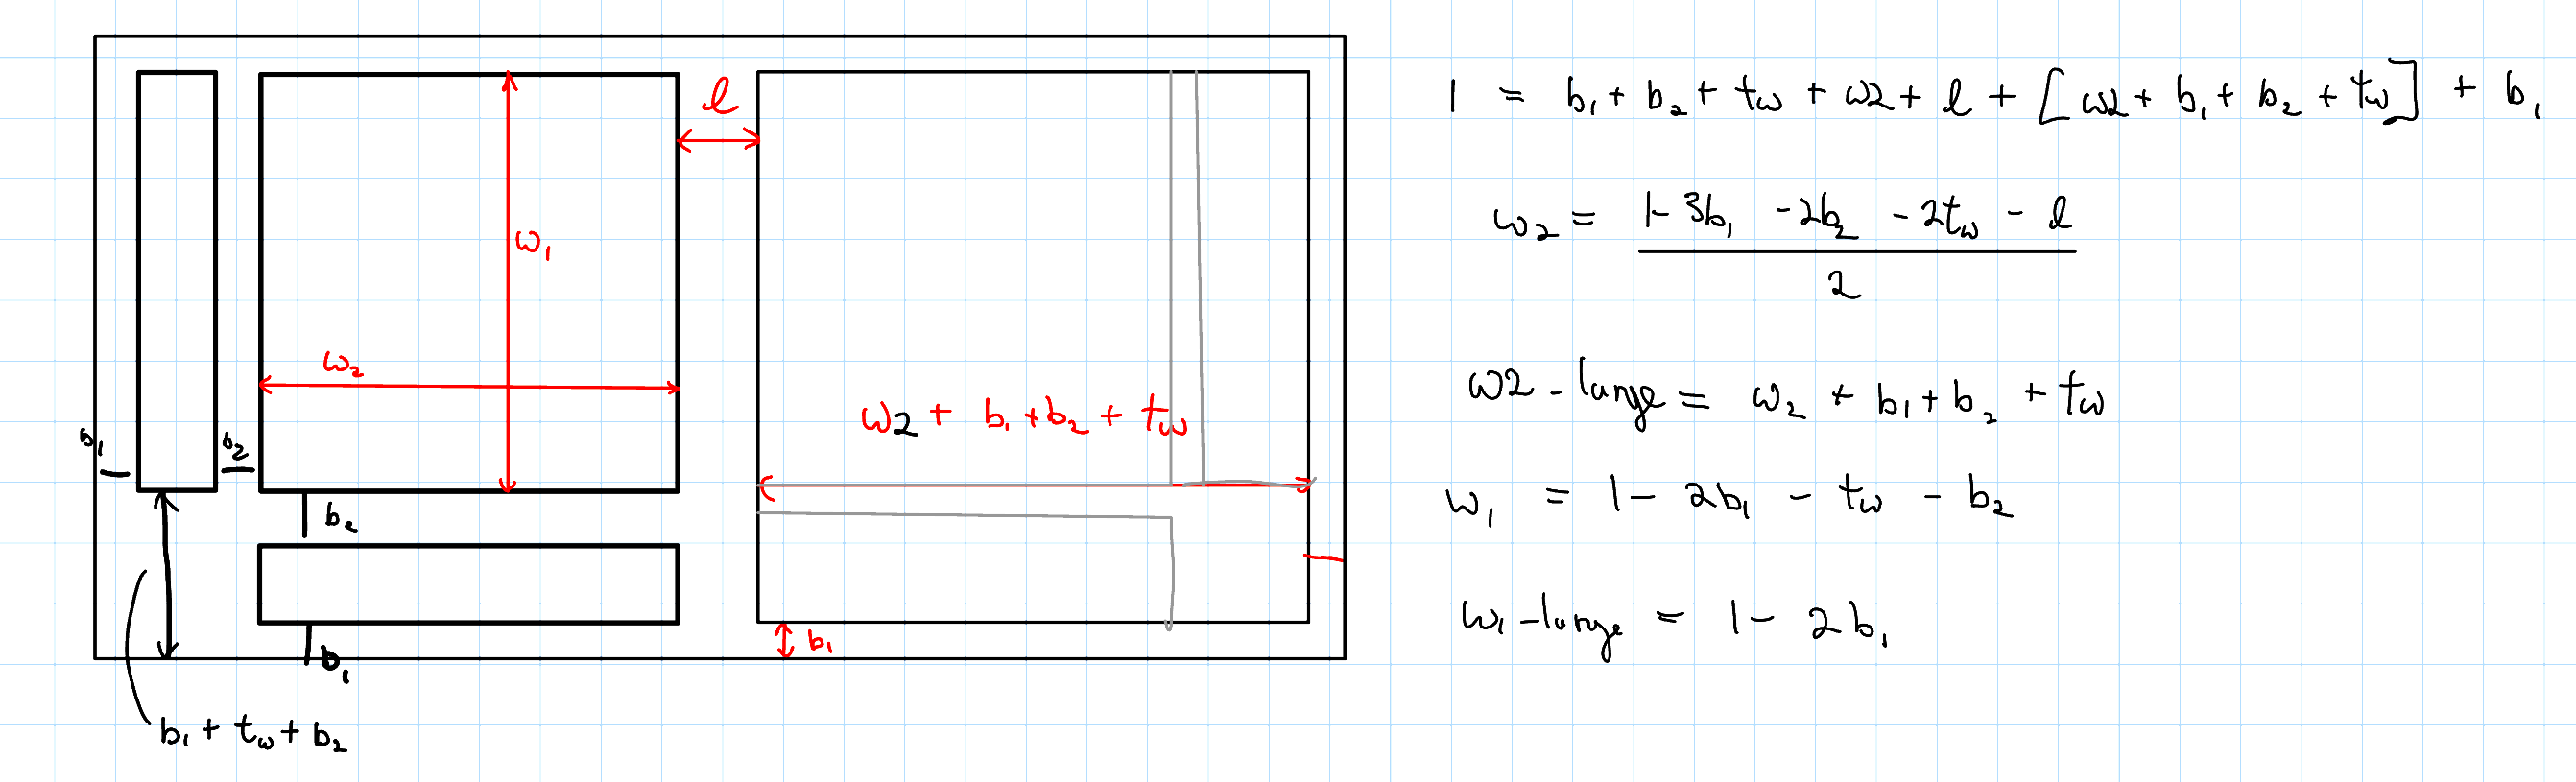
\includegraphics{chapter_05/figs_05/layout_sketch.png}
\caption[{Rough sketch for layout with add\_axese()}]{\textbf{Sketch for
layout with add\_axese().}}
\label{fig:layout_sketch}
\end{figure}
}

\hypertarget{bisect-method}{%
\subsubsection{\texorpdfstring{\texttt{bisect()}
method}{bisect() method}}\label{bisect-method}}

\hypertarget{aph-138-homework-assignment}{%
\section{Aph 138 Homework
Assignment}\label{aph-138-homework-assignment}}

In March of 2022, Matthew Shaw was a guest lecturer for the Quantum
Hardware and Techniques course (APh/Ph 138b). The following is a
homework assignment I wrote to accompany his series of lectures.

The first problem is inspired by the low dark count rate
publication\autocite{Mueller:21}. It has the student build a simple
model for a dark count rate transmitted through a series of filters.
Finally, it leads the student to consider an ultimate tradeoff between
dark count rate and coupling efficiency to wide bandwidth optical
signals. A filtering system that only transmits a very narroband signal
will not be able to detect ultra-short optical signals with high
efficiency or temporal resolution.

The second problem explores a potential use case of a photon number
resolving SNSPD. It closely follows logic presented in an Andreas Christ
and Christine Silberhorn paper\autocite{Andreas:12}. I studied this
paper earlier in my PhD, when I considered developing a multiplexed
single photon source. It turned out that project was overly ambitious,
but future PhD students might consider approaching it again.

{\color{midnightblue} Contact
\href{mailto:andrewstermueller@gmail.com}{Andrew Mueller} with any
questions about the homework or solution manual. The solutions to some
sections specify finer-grained point values when there are multiple
answers per section. As the grader, feel free to use these or not. }

\hypertarget{free-space-coupling-with-low-dark-counts-50-points}{%
\subsection{1. Free space coupling with low dark counts (50
points)}\label{free-space-coupling-with-low-dark-counts-50-points}}

An experimental apparatus emits a collimated beam of
\(1550~\mathrm{nm}\) photons with gaussian beam waist
\(w_0 = 3~\mathrm{mm}\). You wish to focus the beam onto an SNSPD
directly through a window in a cryostat.

\hypertarget{fig:cryostat_concept}{%
\begin{figure}
\centering
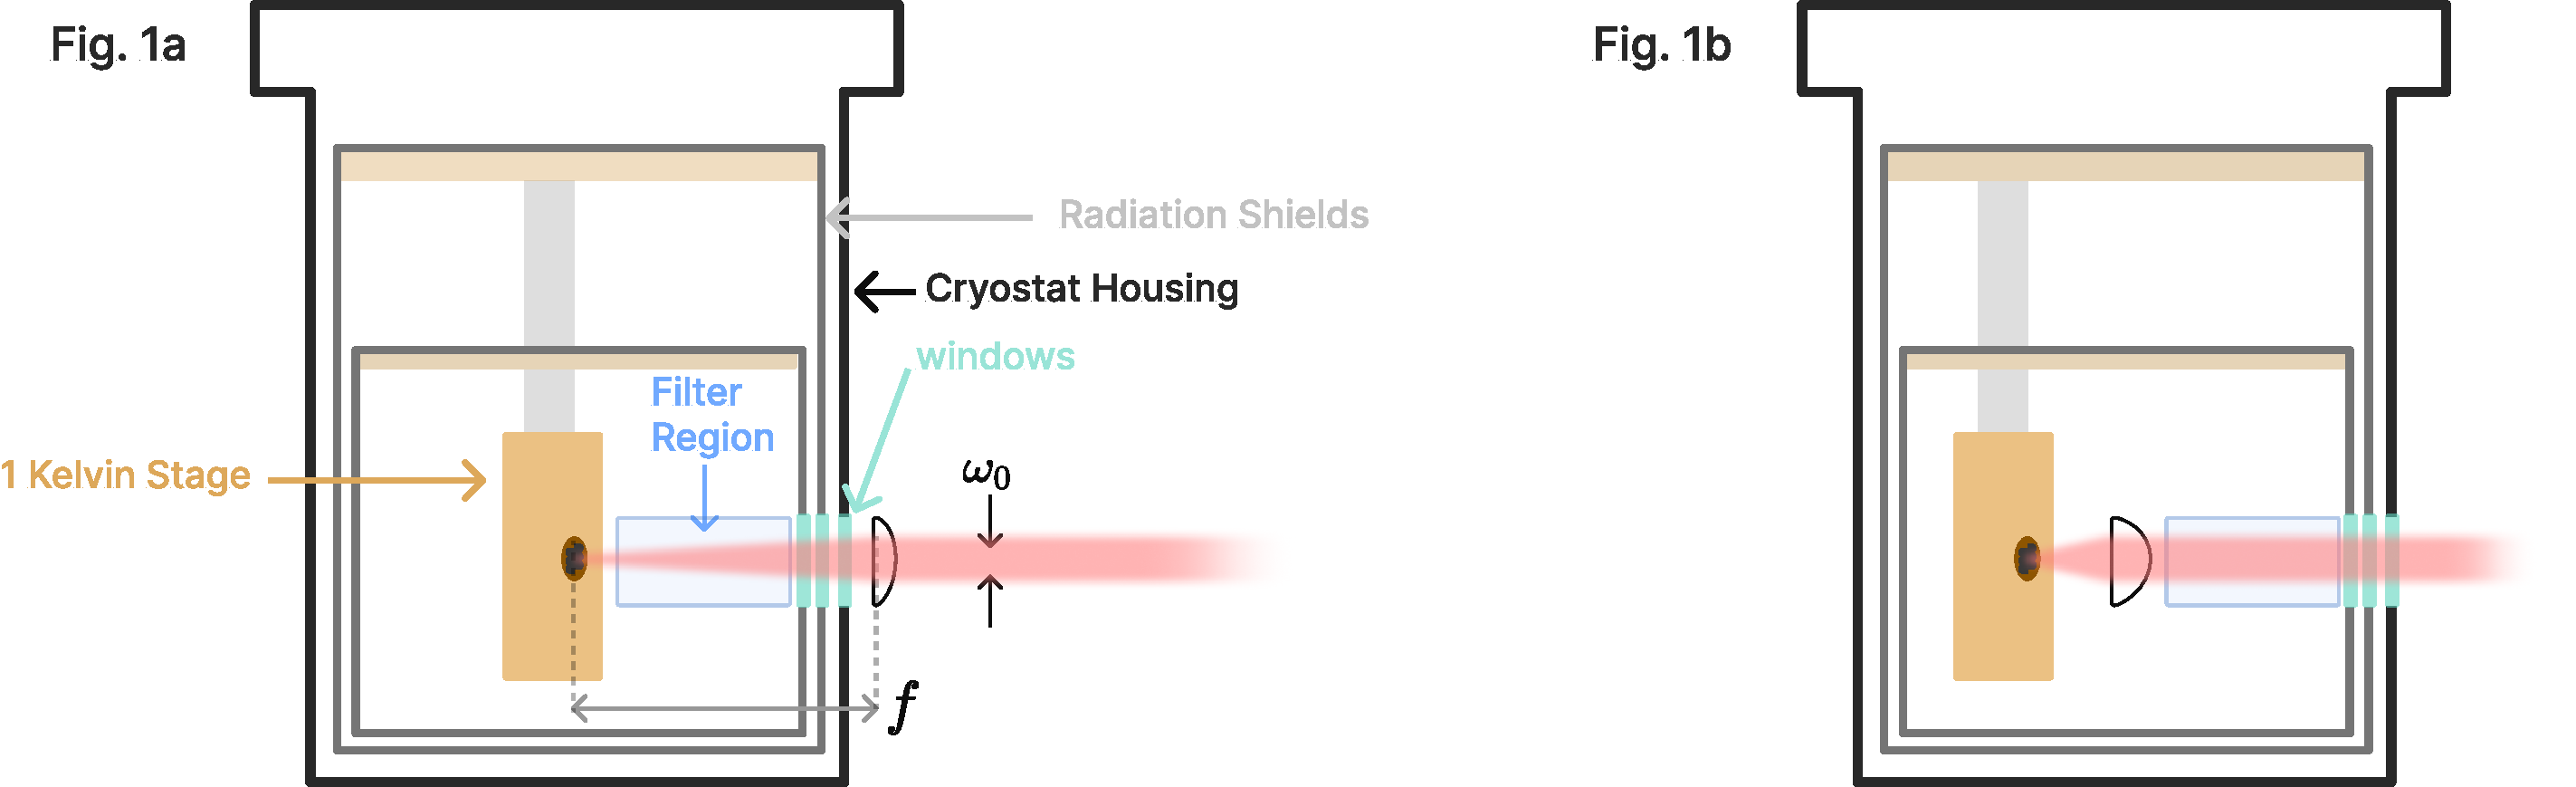
\includegraphics{chapter_05/figs_05/fig1b_light.pdf}
\caption[{Cryostat optical coupling}]{\textbf{Cryostat free space
coupling options.}}
\label{fig:cryostat_concept}
\end{figure}
}

As we will see later on, a set of filters will be needed between the
detector and the window to minimize dark counts. In practice, the set of
filters can be quite thick. Say a \(f = 100~\mathrm{mm}\) lens is used
right outside the cryostat to focus the beam onto the detector though a
set of filters (Fig.~\ref{fig:cryostat_concept} a). The long focal
length makes room for a few inches of filters between the external lens
and focused spot.

\begin{enumerate}
\def\labelenumi{\arabic{enumi}.}
\item
  (4 pts) If the detector has a circular active area with radius
  \(5~\mathrm{\upmu m}\), what ratio of power in the beam can it
  collect? Assume the detector has unity efficiency across all angles of
  incidence with respect to the surface normal.

  {\color{midnightblue}  \textbf{Answer:} } {\color{midnightblue}  The
  divergence angle of the guassian beam:
  \(\theta = \tan^{-1}({\frac{3}{100}})\). }

  {\color{midnightblue}  The formula for divergence angle in terms of
  waist \(w_0\): \(\theta = \frac{\lambda}{\pi w_0}\) }

  {\color{midnightblue}  Combining and plugging in, the waist radius at
  focus is
  \(\frac{1550~\mathrm{nm}}{\pi \tan^{-1}(\frac{3}{100})} \approx 16.5~ \mathrm{\upmu m}\)
  }

  {\color{midnightblue}  The formula for power inside an aperture at
  \(w(z)\) for a guassian beam:}

  {\color{midnightblue} 

  \[P(r, z)=P_{0}\left[1-e^{-2 r^{2} / w^{2}(z)}\right]\]

  }

  {\color{midnightblue} We are interested in the ratio of power
  collected at \(w(z=0) = w_0\) which may be expressed as:}

  {\color{midnightblue} 

  \[P(r, z=0)=1-e^{-2 r^{2} / w_0^{2}}\]

  }

  {\color{midnightblue} Plugging in: }

  {\color{midnightblue} 

  \[P(r, z=0)=1-e^{-2(5^{2}) / 16.5^{2}} \approx  \boxed{0.17} \]

  }
\item
  (4 pts) A faster lens mounted much closer to the detector inside the
  cryostat focuses to a smaller waist. Consider an
  \(f = 18~\mathrm{mm}\) lens with the detector at the focal length
  (Fig.~\ref{fig:cryostat_concept} b). Verify more than 99\% of the
  collimated light will be focused onto the active area of the detector.

  {\color{midnightblue}  The waist radius at focus is
  \(\frac{1550~\mathrm{nm}}{\pi \tan^{-1}(\frac{3}{18})} \approx 2.98~\mathrm{\upmu m}\)
  }

  {\color{midnightblue} Ratio of power within the
  \(10~\mathrm{\upmu m}\) radius active area: }

  {\color{midnightblue} 

  \[P(r, z=0)=1-e^{-2(5^{2}) / 2.98^{2}} \approx \boxed{0.996} \]

  }

  Without filtering, the mid-infrared photons coupled to the detector
  from the room temperature laboratory are a dominant source of dark
  counts. Think of the environment outside the window as an isotropic
  blackbody emitter. Consider 3 cases, where the shaded red regions
  illustrate the light field of thermal radiation that could couple to
  the detector:

  \hypertarget{fig:coupling_options}{%
  \begin{figure}
  \centering
  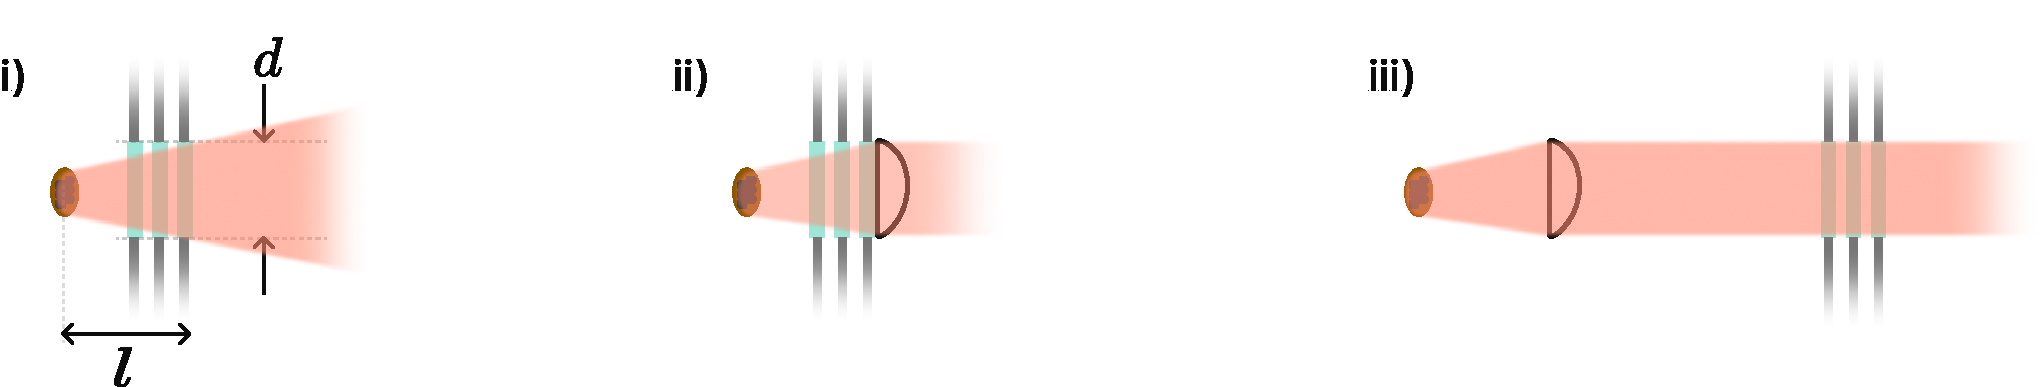
\includegraphics{chapter_05/figs_05/fig2b_light.pdf}
  \caption[{Cryostat coupling options}]{\textbf{Three Coupling Options}}
  \label{fig:coupling_options}
  \end{figure}
  }

  \begin{enumerate}
  \def\labelenumii{\roman{enumii})}
  \tightlist
  \item
    There is no lens; the detector is distance \(l\) inside the
    cryostat, and the first window with diameter \(d\) defines an
    entrance pupil.
  \item
    Same as (i), but a lens with focal length \(l\) is placed right
    outside the first window. The detector is at the focal point.
  \item
    Same as (ii) but the lens is placed inside the cryostat with the
    detector still at the focal length. Equivalent to
    Fig.~\ref{fig:cryostat_concept} b above.
  \end{enumerate}
\item
  (6 pts) Does (ii) couple more, less, or equal dark counts to the
  detector than (i)? What about case (iii)? Why? No calculations should
  be needed. (Hint: Consider the units of radiance, which characterizes
  a black body emitter. Etendue or beam parameter product may be useful
  concepts to consider)

  {\color{midnightblue}  \textbf{Answer:} } {\color{midnightblue}  The
  three cases couple the same amount of light to the detector. (ii)
  couples the same amount of power as (i) because a blackbody source
  can't be focused to higher intensity with a lens. The solid angle
  subtended by the entrance pupil as seen by the detector is the same in
  all cases. The detector area stays the same as well so the etendue is
  conserved across all three cases. This implies the same radiant power
  is coupled. }

  {\color{darkred}  3 points for saying all situations couple the same
  rate; 3 points for some explanation. }
\item
  (9 pts) Using Planck's law with laboratory temperature \(T\) and the
  geometry of case (i) above, write an expression for spectral radiant
  flux (photons per unit wavelength) on the active area of a detector
  with radius \(r\).

  {\color{midnightblue}  \textbf{Answer:} } {\color{midnightblue} The
  expression is a product of several factors:}

  {\color{midnightblue} 

  \[\text{Flux}[\lambda] = P \Omega D_{area} B_{\lambda}(\lambda, T)\]

  }

  {\color{midnightblue}  Where \(P = \frac{\lambda}{hc}\) is the number
  of photons per unit energy, \(\Omega\) is the solid angle of blackbody
  radiation as seen by the detector, \(D_{area} = \pi r^2\) is the area
  of the detector, and \(B_{\lambda}\) is Planck's law. }
  {\color{midnightblue} Planck's law:}

  {\color{midnightblue} 

  \[B_{\lambda}(\lambda, T)=\frac{2 h c^{2}}{\lambda^{5}} \frac{1}{e^{h c /\left(\lambda k_{\mathrm{B}} T\right)}-1}\]

  }

  {\color{midnightblue}  \(\Omega = \pi \sin{\theta^2}\), where
  \(\theta = \tan^{-1}(\frac{(d/2)}{l})\) is the half angle of the field
  of view of blackbody radiation as seen by the detector. }

  {\color{midnightblue} The full expression: }

  {\color{midnightblue} 

  \[\text{Flux}[\lambda] = \frac{\lambda \pi^2 r^2 \sin{\theta^2}}{hc} \frac{2 h c^{2}}{\lambda^{5}} \frac{1}{e^{h c /\left(\lambda k_{\mathrm{B}} T\right)}-1}, \,\,\,\,\,\,\,\,\,\,\,\theta = \tan^{-1}(\frac{(d/2)}{l})\]

  }

  {\color{midnightblue}  Since the expression asked for can be written
  many ways, just verify the student has taken into account all the
  terms in equation (1) above, and has the correct expressions for}
  {\color{darkred} \(\Omega\) (3 pts), \(\theta\) (3 pts), and P (3
  pts).}
\item
  (6 pts) Consider the configuration in Fig. 1b). The detector has an
  internal quantum efficiency approximated by:

  \[\eta(\lambda) = \frac{1}{2}(1 - \text{erf}[\lambda - 3~\mathrm{\upmu m}]) \]

  \(\lambda\) is measured in \(\mathrm{\upmu m}\) and \(\text{erf}()\)
  is the error function. Using your conclusions from (1.3) and
  expression from (1.4), write a formula \(N_{photons}[\lambda]\) for
  the number of detectable dark counts with respect to \(\lambda\), then
  numerically integrate it to find the dark count rate with no
  filtering. The laboratory temperature \(T\) is 293 K, lens focal
  length \(l\) is \(18~\text{mm}\), detector radius \(r\) is
  \(5~\mathrm{\upmu m}\), and the diameter \(d\) of all optics is 1
  inch. The maximum count rate of this SNSPD is 10 MHz. Is the detector
  usable or overexposed?

  {\color{midnightblue}  \textbf{Answer:} } {\color{midnightblue} Use
  the expression from (1.4) and multiply it by the quantum efficiency
  function \(\eta(\lambda)\) }

  {\color{midnightblue} 

  \[N_{photons}[\lambda] = P \Omega D_{area} \eta(\lambda) B_{\lambda}(\lambda, T=293)\]

  }

  {\color{midnightblue}  Here is the function expressed in mathmatica
  and the solution to the integral: }

  {\color{midnightblue} 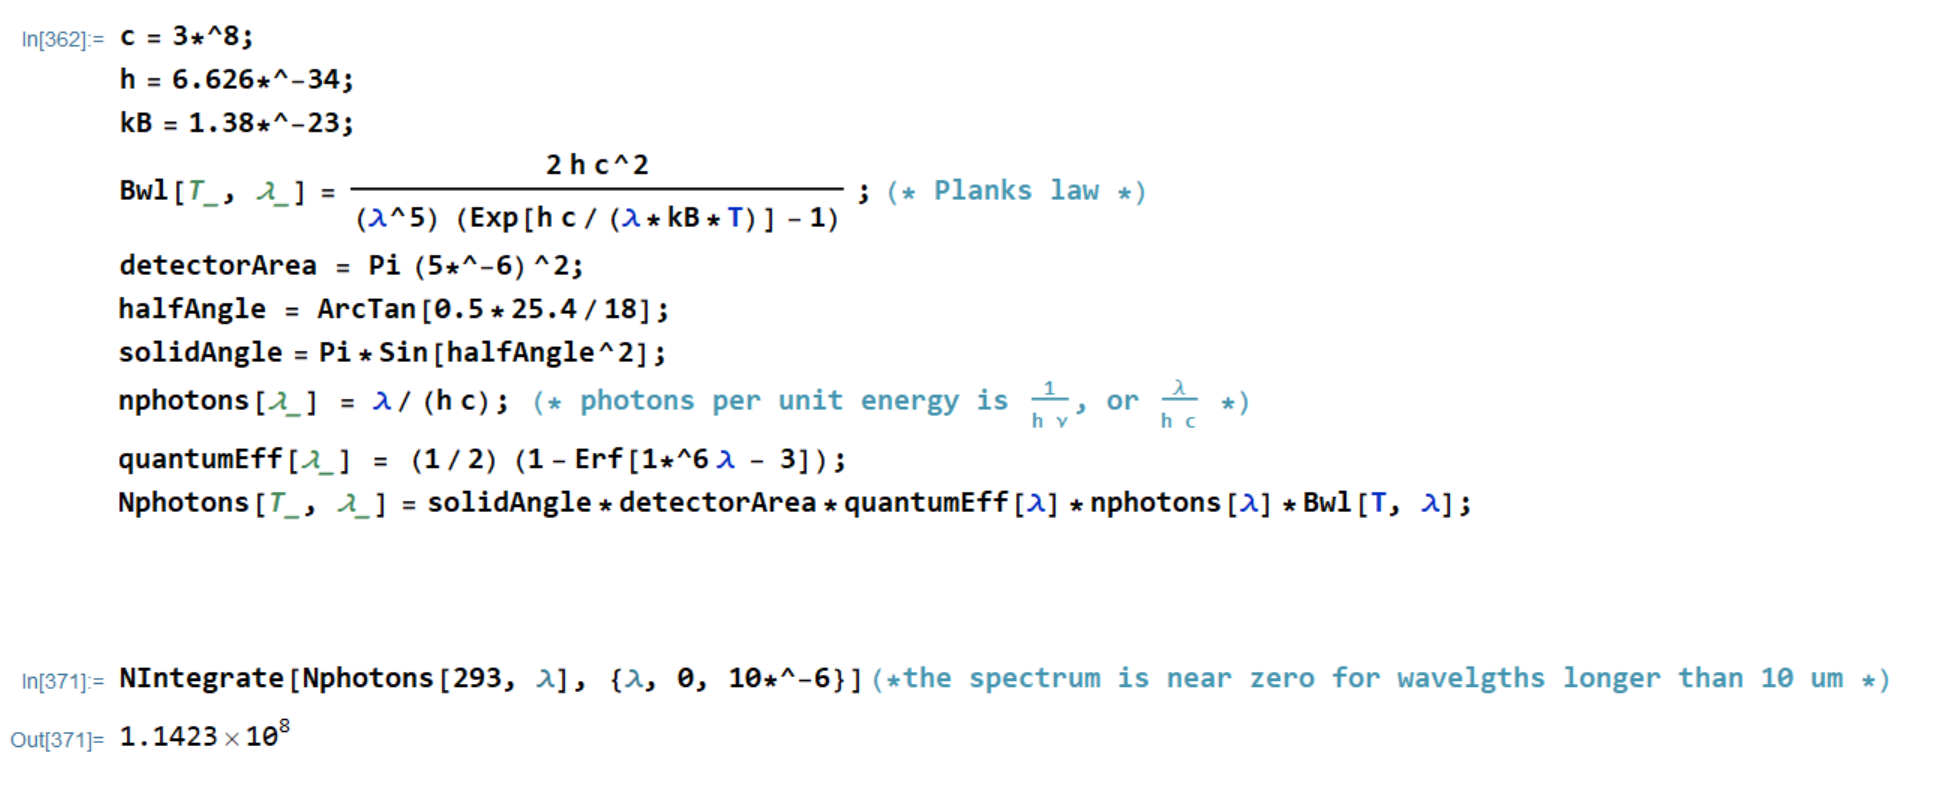
\includegraphics{chapter_05/figs_05/mathematica_2.PNG}}

  {\color{midnightblue} Dark count rate
  \(\approx \boxed{110 \,\text{MCounts/s}}\) } {\color{midnightblue} The
  rate of dark counts exceeds the usual maximum count rate, the detector
  is not usable. }

  {\color{darkred} 3 pts. for similar dark count rate (+/- 20\%) , 3
  pts. for saying the detector is not usable.}
\item
  (6 pts) A set of shortpass filters can remove the bulk of blackbody
  radiation. A shortpass filter can be roughly modeled with the formula:

  \[F(\lambda, E_t) = \frac{1}{E_t}[(E_t - 1)H(\lambda_c - \lambda) + 1]\]

  Where H is the Heaviside step function, \(\lambda_c\) is the cutoff
  wavelength of the filter, and \(E_t\) is the extinction ratio of the
  filter. Use this with \(N_{photons}[\lambda]\) from (d). How many
  filters with \(\lambda_c = 1560~\text{nm}\) and \(E_t = 30~\text{dB}\)
  are necessary to suppress the spectral region of detectable dark
  counts longer than 1560 nm so that it is not the dominant source of
  dark counts?

  {\color{midnightblue}  \textbf{Answer:} }

  {\color{midnightblue} \(\boxed{\text{3 filters}}\) are needed to make
  the wavelength band shorter than 156 nm the dominant source of
  counts.} {\color{darkred} 3 pts. for this answer}

  {\color{darkred} 3 pts for evidence:} {\color{midnightblue} Students
  might integrate the detectable dark count spectrum with different
  numbers of filters and comparing the results. The computations below
  show the addition of a fourth filter has a negligible effect on the
  dark count rate. }

  {\color{midnightblue} Students may instead give a more qualitative
  answer, for example with a graph of the filtered spectrums, that shows
  the relative suppression of the region longer than 1560 nm. }

  {\color{midnightblue} 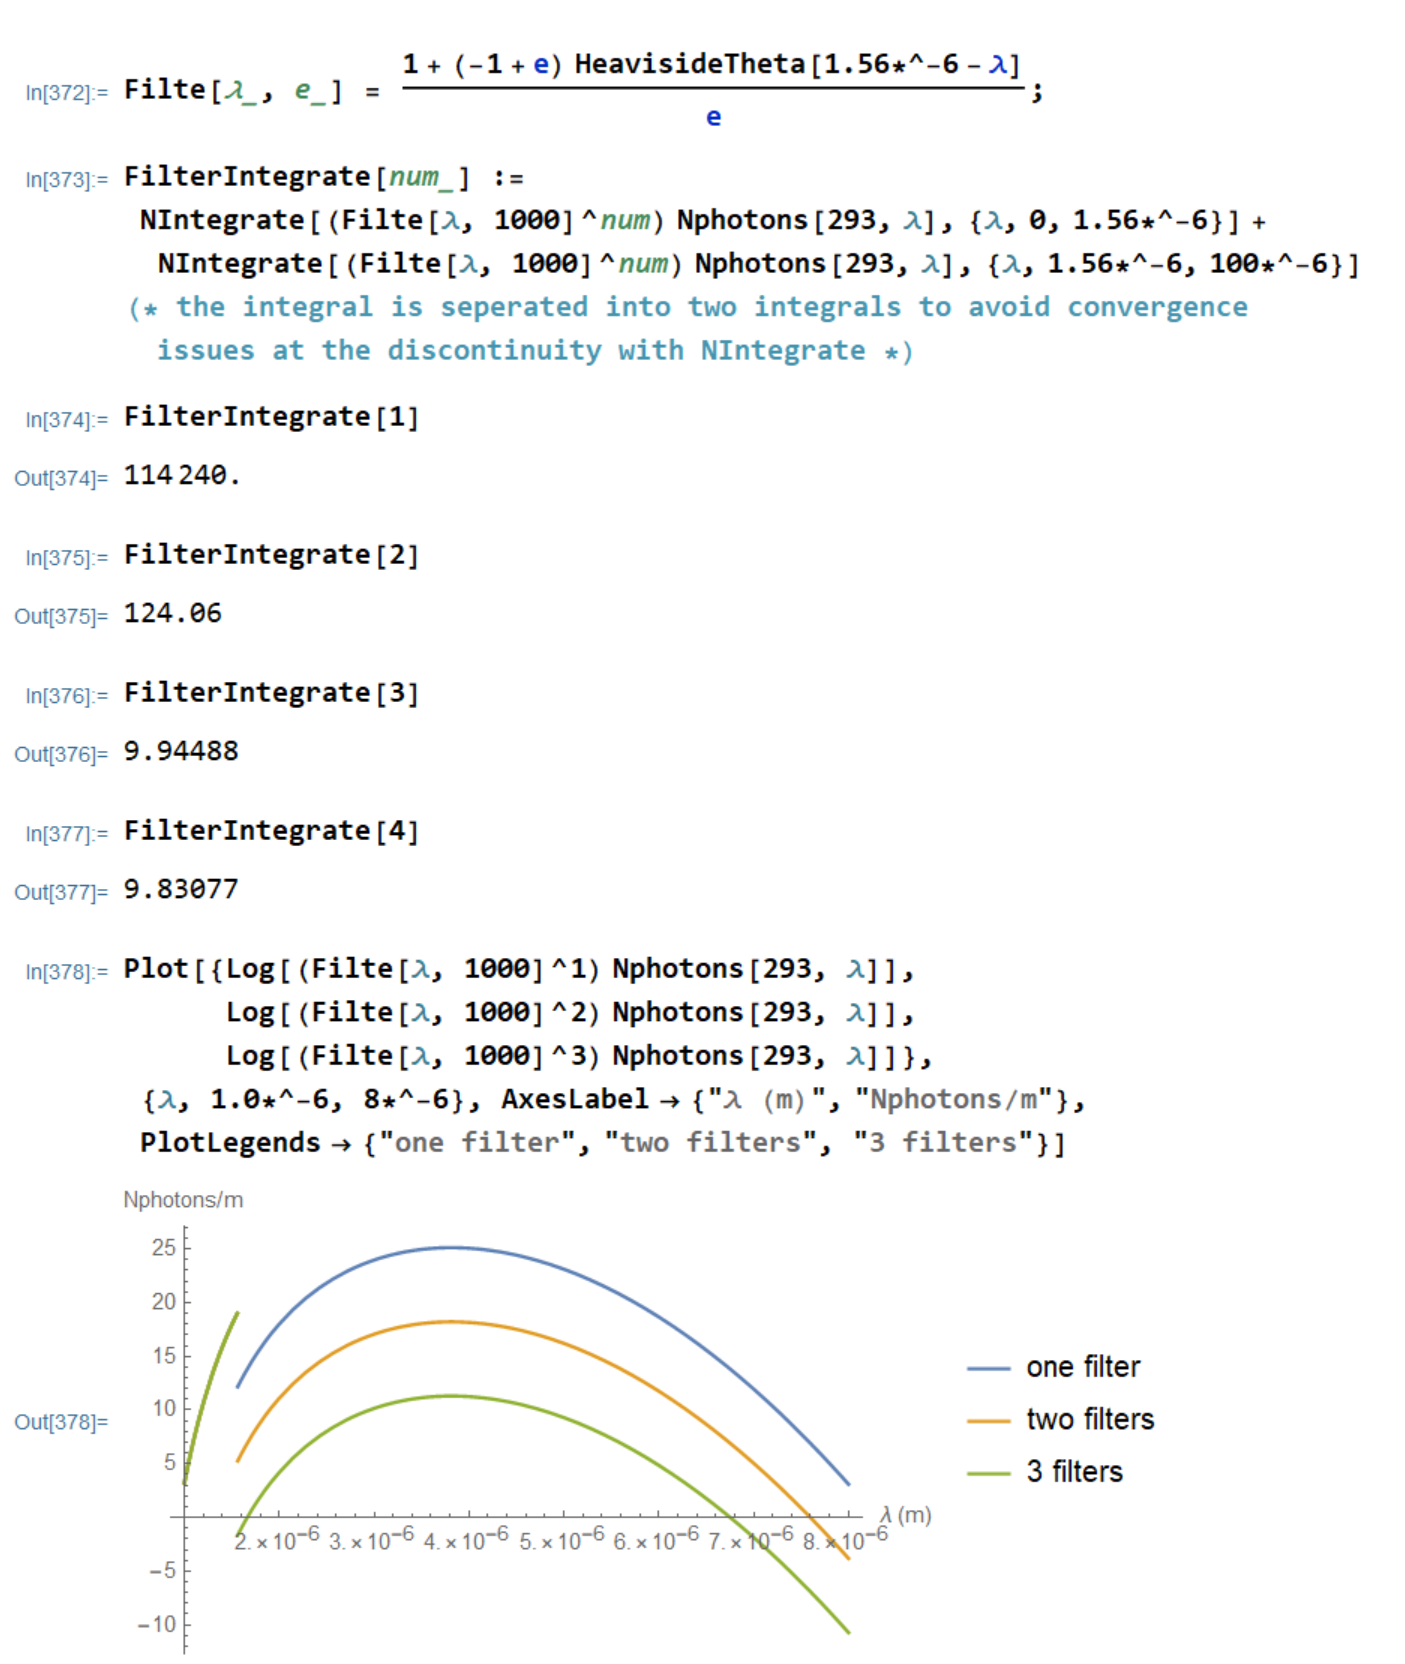
\includegraphics{chapter_05/figs_05/filter_integrate_4.PNG}}
\item
  (7 pts) If a narrow band filter is also inserted with center
  wavelength \(1550~\text{nm}\) and spectral width below \(1-2~nm\),
  then dark count rate can be approximated as just
  \(N_{photons}[\lambda = 1550~\text{nm}]\) times the filter width. Show
  for this wavelength range you can simplify dark count rate further to
  a simple exponential function. If the laboratory air conditioner
  breaks, raising the lab temperature from 293 K to 300 K, how much
  higher is the dark count rate?

  {\color{midnightblue}  \textbf{Answer:} }

  {\color{midnightblue} The expression for \(N_{photons}[\lambda]\) from
  part (1.4) can be simplified and evaluated at 1550 nm, then multiplied
  by the filter width in nanometers. }

  {\color{midnightblue} 

  \[\begin{aligned}
   N_{photons}[\lambda] &= P \Omega D_{area} \eta(\lambda) B_{\lambda}(\lambda) \\
   N_{filter} &= N_{photons}[\lambda = 1550~\text{nm}]\Delta \lambda
   \end{aligned}\]

  }

  {\color{midnightblue} This code shows integrating the spectrum and
  just multiplying \(N_{photons}\) times the filter width produce very
  similar results (for a 1 nm filter):}

  {\color{midnightblue} 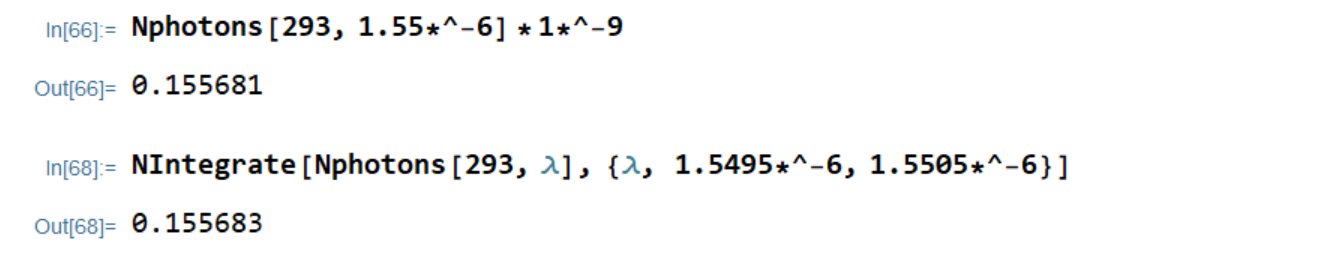
\includegraphics{chapter_05/figs_05/nphoton_approx.PNG}}

  {\color{midnightblue} Evaluating the \(N_{photon}\) function at
  \(\lambda = 1550~text{nm}\) shows the \(-1\) term is small relative to
  the exponential term:}

  {\color{midnightblue} 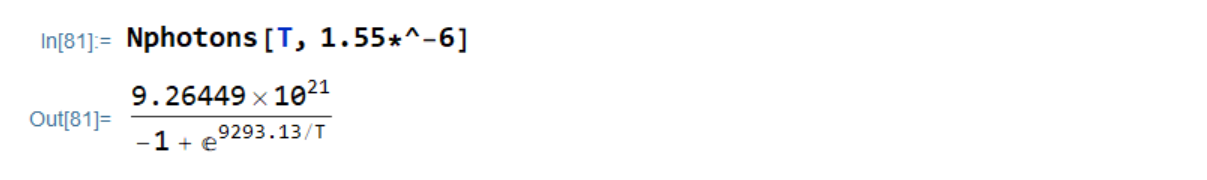
\includegraphics{chapter_05/figs_05/small_relative_to_exponential.PNG}}

  {\color{midnightblue} Therefore the filter transmission approximation
  is:}

  {\color{midnightblue} 

  \[\boxed{N_{filter} \approx 9.26\mathrm{e}21 \Delta\lambda e^{-9290/T} (\frac{\text{photons}}{\text{s*meter}})}\]

  }

  {\color{midnightblue} or equivalently: }

  {\color{midnightblue} 

  \[\boxed{N_{filter} \approx 9.26\mathrm{e}12 \Delta\lambda e^{-9290/T} (\frac{\text{photons}}{\text{s*nm}})}\]

  }

  {\color{midnightblue} and the dark count rate in the 300 K room is
  roughly double the rate in the 293 K room: }

  {\color{midnightblue} 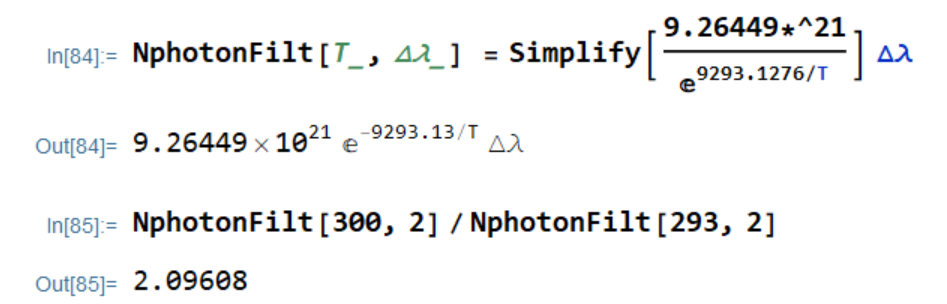
\includegraphics{chapter_05/figs_05/filter_with_temp.PNG}}

  {\color{darkred} 4 pts for a similar equation, 3 pts for finding the
  dark count rate roughly doubles. }

  A quantum communication experiment requires time-tagging photons with
  respect to a 50 GHz clock with 95\% fidelity. That is, 95\% of the
  timing measurements of detected photons emitted at the same time with
  respect to a clock fall within a 20 ps bin. Say the detector and
  readout electronics have a combined jitter of 10 ps FWHM, and a mode
  locked laser is used for the experiment that generates
  transform-limited Gaussian pulses. You tune it's temporal length to a
  value for which the total timing uncertainty of time-tagged photons
  --- including system jitter and pulse temporal length --- matches the
  95 \% fidelity at 50 GHz requirement. Assume detector jitter has a
  Gaussian shape as well.
\item
  (8 pts) Find the spectral width of a filter that would transmit 95\%
  of the photons from the mode locked laser. What is the dark count rate
  with this filter, using the expression from (1.7) and T = 293 K?

  {\color{midnightblue}  \textbf{Answer:} }

  {\color{midnightblue} For transform limited guassian pulses, the
  product of temporal and spectral width at a FWHM level is
  \href{https://www.lasercalculator.com/transform-limited-pulse-calculator/}{about
  0.441}. There's a derivation of this
  \href{https://www.physicsforums.com/threads/time-bandwidth-product-ideal-mode-locking.171404/post-1339948}{here},
  but students don't need to show it. }

  {\color{midnightblue} 

  \[T B P_{\text {Gaussian }}=\frac{2 \log 2}{\pi} \approx 0.441\]

  }

  {\color{midnightblue}  Since this uses the FWHM level, all the 95\%
  metrics need to be converted. About 95\% of the area under a guassian
  falls within \(\pm 2 \sigma\). }

  {\color{midnightblue}  Bound on total system timing uncertainty:
  \(20~\text{ps}_{95\%} = (20/4)*2.35 = 11.75~\text{ps}_{FWHM}\) }

  {\color{midnightblue}  The jitter of the detection system and the
  temporal width of the laser pulse \(\Delta t\) should add in
  quadrature to match the bound: }

  {\color{midnightblue} 

  \[ 11.75~\text{ps}_{FWHM} = \sqrt{ \Delta t^2 + (10~\text{ps})^2}\]

  }

  {\color{midnightblue} 

  \[ 0.441 = \Delta t \Delta \nu \] \[\Delta \nu = 71~\text{GHz}\]
  \[\Delta \lambda = \frac{\lambda^2 \Delta \nu}{c} = 0.57~\text{nm}\]

  }

  {\color{midnightblue}  \(0.57~\text{nm}\) is the spectral width of the
  laser pulse at the FWHM level. If this pulse passes through a tophat
  filter with width equal to the 95\% level of the laser pulse, then
  95\% will be transmitted. }

  {\color{midnightblue} Filter width: }

  {\color{midnightblue} 

  \[\Delta \lambda_{95\%} = \frac{4 \Delta \lambda}{2.35} \approx \boxed{1~\text{nm}} \]

  }

  {\color{midnightblue} Dark count rate is easy to find using the
  expression from the previous section: }

  {\color{midnightblue} 

  \[\boxed{N_{filter} \approx 9.26e12 (1~\text{nm}) e^{-9290/T} (\frac{\text{photons}}{\text{s*nm}})} \approx 0.15~\text{photons/s} \]

  }

  {\color{darkred} 3 points for writing and solving the equation that
  matches the jitter bound to the quadrature sum } {\color{darkred} 5
  points for correct filter width and dark count rate}
\end{enumerate}

\hypertarget{spdc-coupling-and-single-photon-sources-50-points}{%
\subsection{2. SPDC Coupling and Single Photon Sources (50
points)}\label{spdc-coupling-and-single-photon-sources-50-points}}

A Spontaneous Parametric Down Conversion (SPDC) crystal is known to
generate a twin beam squeezed state of the form:

\[|\psi\rangle= \sqrt{1 - \gamma^2} \sum_{n=0}^{\infty} \gamma^{n}\left|n_{s}, n_{i}\right\rangle \]

Where \(n_s\) and \(n_i\) are the number of photons corresponding to the
signal and idler parts of the wavefunction. Consider Fig.~\ref{fig:hsps}
a, where the crystal is pumped with a pulsed laser, and the the signal
and idler components that emerge are separated either by polarization or
frequency. The idler arm is sent to an SNSPD. This configuration can be
used as a heralded single photon source (HSPS). A click on the detector
on the idler arm `heralds' a non-vacuum state in the signal arm. High
fidelity and probability single photon sources are very useful for
various quantum optics experiments and technologies, including linear
optical quantum computing.

\hypertarget{fig:hsps}{%
\begin{figure}
\centering
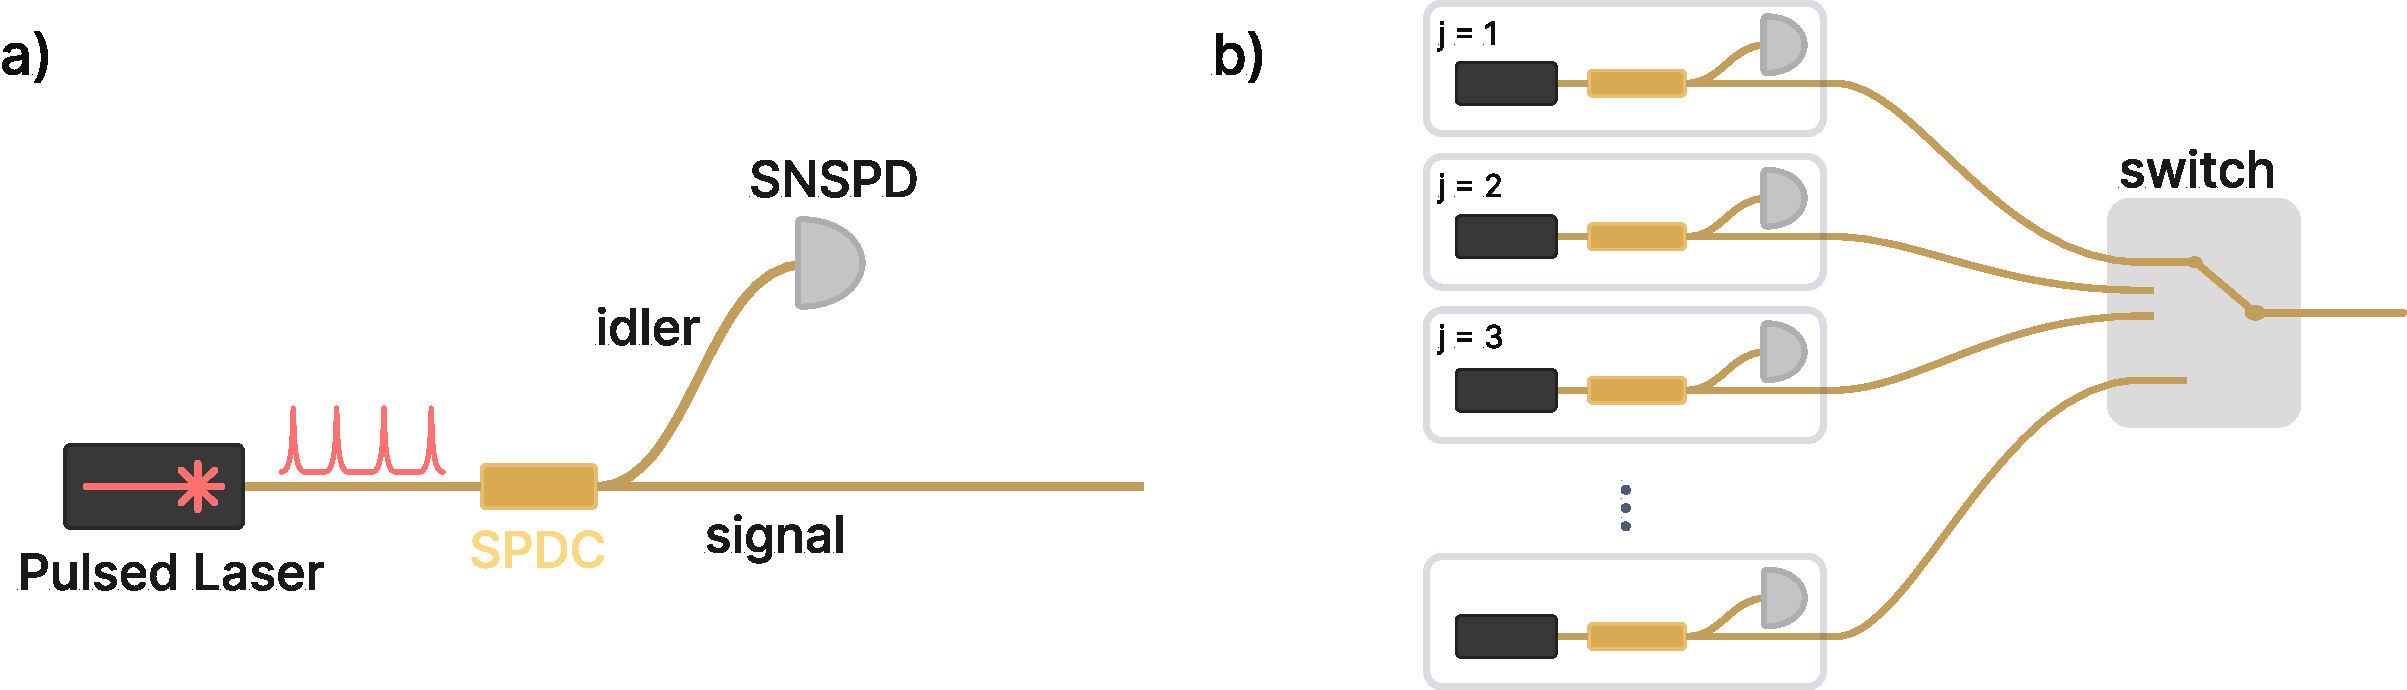
\includegraphics{chapter_05/figs_05/hsps_light.pdf}
\caption[{Heralded single photon source designs}]{\textbf{Heralded
single photon sources}}
\label{fig:hsps}
\end{figure}
}

Most SNSPDs are \emph{binary}-type single photon detectors, meaning they
differentiate between zero and one or more photons arriving in a given
light pulse. A positive operator value measure (POVM) quantifies how a
`click' from a binary SPD updates our knowledge of the incident state:

\[\hat{\Pi}_{\text {binary}} = \sum_{n=0}^{\infty}\left[1-(1-\eta)^{n}\right]|n\rangle\langle n|\]

Where \(\eta\) is the coupling efficiency between the state of interest
and the detector.

\begin{enumerate}
\def\labelenumi{\arabic{enumi}.}
\item
  (6 pts) Find the expectation value of \(\hat{\Pi}_{\text {binary}}\)
  given the SPDC state above. This is the probability
  \(p_{binary}\left(\gamma, \eta\right)\) of getting a binary detector
  click on the idler arm. For \(\gamma << 1\), what is \(p_{binary}\) up
  to lowest order in \(\gamma\), and what fock state of the signal arm
  is the source of this dominant term?

  {\color{midnightblue}  \textbf{Answer:} }

  {\color{midnightblue} 

  \[\begin{aligned}
   \langle \psi | \Pi_{\text {binary}} | \psi \rangle &= (1- \gamma^2) \sum_{\tilde{n}=0}^{\infty} \langle \tilde{n}_s \tilde{n}_i | \gamma^{\tilde{n}} \sum_{n=0}^{\infty}[1 - (1-\eta)^{n}] \gamma^n | n_s n_i \rangle \\
   \langle \psi | \Pi_{\text {binary}} | \psi \rangle &= p_{binary}(\gamma, \eta) =  \boxed{(1-\gamma^2) \sum_{n_s=0}^{\infty} \gamma^{2n_s} [1 - (1 - \eta)^{n_s}]}
   \end{aligned}\]

  }

  {\color{midnightblue} For
  \(\gamma << 1, ~~ p \sim (1 - \gamma^2)[\cancel{\gamma^0[1 - (1 - \eta)^0]} + \gamma^{2}\eta ] \sim (1 - \gamma^2)\gamma^{2}\eta\)
  }

  {\color{midnightblue}  To lowest order in \(\gamma\),
  \(p \sim \gamma^{2}\eta\). The single photon fock state dominates for
  \(\gamma << 1\). }

  {\color{darkred}  3 pts for correct \(p_{binary}(\gamma, \eta)\); 3
  pts for saying the leading term is from single photons }
\item
  (6 pts) A general form for the density matrix of the signal mode given
  a herald event is:

  \[\rho_{s}\left(\gamma, \eta\right)=\frac{\operatorname{Tr}_{i}\left(\hat{\Pi}|\psi\rangle\langle\psi|\right)}{\left\langle\psi\left|\hat{\Pi}\right| \psi\right\rangle}\]

  Write down the \(|1\rangle\langle1|\) term of this matrix, and
  simplify any infinite sums. This is the single photon fidelity
  \(F_{binary}(\gamma, \eta)\). Why does \(F_{binary}\) approach zero
  for \(\gamma\) approaching 1? What types of states is the SPDC
  generating in this limit?

  {\color{midnightblue}  \textbf{Answer:} }

  {\color{midnightblue} 

  \[\begin{aligned}
   \rho_s(\gamma,\eta) &= \frac{\operatorname{Tr}_i[\cancel{(1 - \gamma^2)}\Sigma_{n=0}^{\infty} \gamma^{2n}[1 - (1 - \eta)^{n} ]| n \rangle \langle n | n_s n_i \rangle \langle n_s n_i |]}
   {\cancel{(1-\gamma^2)} \sum_{n_s=0}^{\infty} \gamma^{2n_s} [1 - (1 - \eta)^{n_s}]}\\
   |1_s \rangle \langle 1_s | &= \frac{\gamma^2[1 - (1 - \eta)]}{\sum_{n_s=0}^{\infty} \gamma^{2n_s} [1 - (1 - \eta)^{n_s}]} = \frac{\gamma^2 \eta}{\sum_{n_s=0}^{\infty} \gamma^{2n_s} [1 - (1 - \eta)^{n_s}]}\\
   |1_s \rangle \langle 1_s | &= \frac{\gamma^2 \eta}{\sum_{n_s=0}^{\infty}(\gamma^{2n_s} - [\gamma^2 (1 - \eta)]^{n_s})}\\
   &= \frac{\gamma^2 \eta}{\frac{1}{1 - \gamma^2} - \frac{1}{1 - \gamma^2(1 - \eta)}}\\
   &= \frac{\gamma^2 \eta (1 - \gamma^2)}{1 - \frac{1 - \gamma^2}{1 - \gamma^2(1 - \eta)}}\\
   &= \frac{\cancel{\gamma^2 \eta} (1 - \gamma^2) (1 - \gamma^2 (1 - \eta))}{\cancel{1 - \gamma^2 (1 - \eta) - 1 + \gamma^2}} \\
   F_{binary}(\gamma, \eta) &= \boxed{(1 - \gamma^2)(1 - \gamma^2(1 - \eta))}
   \end{aligned}\]

  }

  {\color{midnightblue} As \(\gamma\) approaches 1, the denominator in
  the original expression for \(\rho_s(\gamma,\eta)\) approaches
  infinity while the numerator approaches \(\eta\). In this limit, the
  SPDC is generating predominantly multi-photon states. For \(\gamma\)
  approaching 1, the probability of the generated state being a single
  photon state goes to zero. Because the binary POVM was used,
  multi-photon states are `included' in \(\rho_s(\gamma,\eta)\). For
  \(\rho_s\) from the PNR POVM shown below, multi-photon states will be
  included to a much lesser extent, depending on the value for
  \(\eta\).}

  {\color{darkred} 3 pts for correct \(F_{binary}(\gamma, \eta)\); 3 pts
  for similar explanation}

  An HSPS with high single photon fidelity and probability is most
  useful, but you see these metrics are maximized for opposite limits of
  \(\gamma\). One approach to achieving high probability and fidelity
  simultaneously is to link multiple SPDC sources and heralding
  detectors as shown in Fig.~\ref{fig:hsps} b. A click from the detector
  \(j\) triggers the switch to move to position \(j\) and let the
  heralded state pass through. This way, \(\gamma\) for each source can
  be kept low to maximize fidelity, while heralding probability
  increases with the number of sources.
\item
  (6 pts) If such a multiplexing setup is engineered to have 98\% single
  photon fidelity from each source and 98\% heralding probability
  overall, how many sources and binary SNSPDs are needed? Use an idler
  arm efficiency \(\eta\) of 80\%.

  {\color{midnightblue}  \textbf{Answer:} }

  {\color{midnightblue} The fist step is to determine the pump power
  \(\gamma\) for which fideltiy is 98\%. }

  {\color{midnightblue} 

  \[0.98 = F_{binary}(\gamma, \eta) = (1 - \gamma^2)(1 - \gamma^2(1 - \eta)\,\,\,\,\,\,\,\, \eta = 0.8\]

  }

  A numerical solution is fine. We're interested in the positive
  solution less than one:

  {\color{midnightblue} 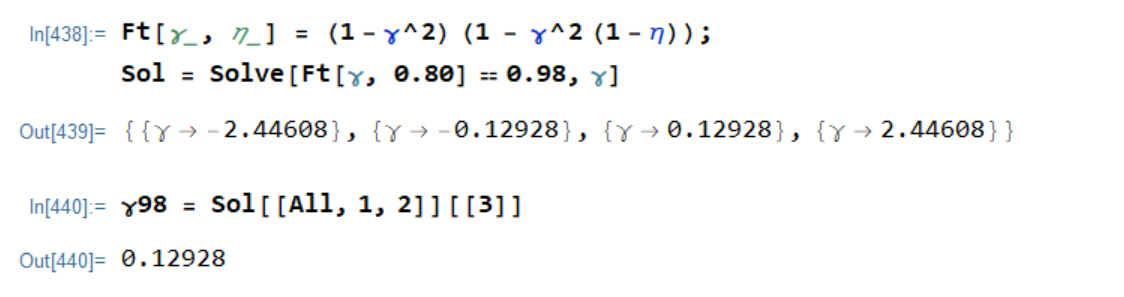
\includegraphics{chapter_05/figs_05/Ftsolve.PNG}}

  {\color{midnightblue} Like in introductory statistics problems, its
  helpful to think about the negative case: Given N sources with herald
  probability \(p\), the probability of zero sources heralding is:}

  {\color{midnightblue} 

  \[P(\text{no herald}|N) = (1 - p_{binary}\left(\gamma, \eta\right))^N\]

  }

  {\color{midnightblue} Then the probability of at least one herald is 1
  minus the previous expression:}

  {\color{midnightblue} 

  \[P(\text{at least one herald}|N) = 1 - (1 - p_{binary}\left(\gamma, \eta\right))^N\]

  }

  {\color{midnightblue} 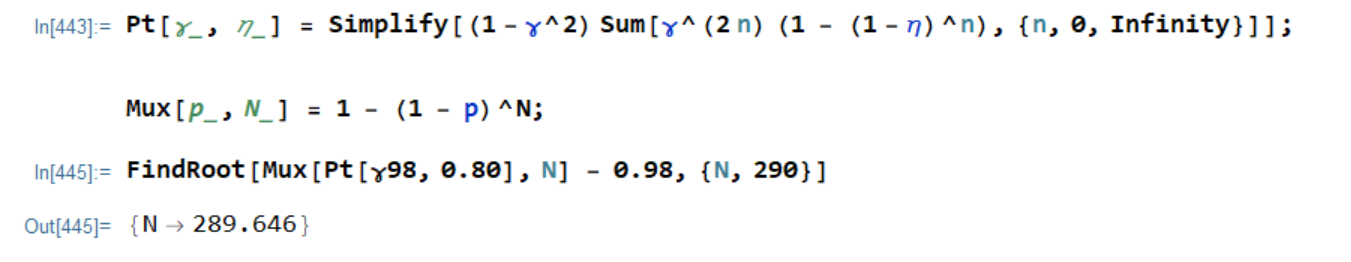
\includegraphics{chapter_05/figs_05/mux_binary.PNG}}

  {\color{midnightblue} About \(\boxed{N = 290}\) sources are needed.}

  {\color{darkred} 3 pts for correct form of the multiplexing expression
  \(P(\text{at least one herald}|N)\); 3 pts for similar number of
  sources \(N\)}
\end{enumerate}

A photon number resolving (PNR) SNSPD is able to discriminate the number
of photons in a light pulse*. By heralding the idler mode with a PNR
SNSPD, the generation of multi-photon signal pulses can be identified
and discarded. There's a POVM for an ideal PNR single photon detector,
where \(i\) is the number of photons detected**:

\[\hat{\Pi}_{PNR}(i)=\sum_{n=i}^{\infty}\binom{n}{i}(1-\eta)^{n-i} \eta^{i}|n\rangle\langle n|\]

\begin{enumerate}
\def\labelenumi{\arabic{enumi}.}
\setcounter{enumi}{3}
\item
  (12 pts) Derive a herald probability \(p_{PNR}\) and fidelity
  \(F_{PNR}\) for the PNR POVM, following the steps in the previous
  sections with \(i\) set to 1. You can use symbolic math tools to
  simplify them if you wish. The probability of successfully heralding
  states in the signal arm \(p_{PNR}\) should now approach zero for
  \(\gamma\) near one. Why is this?

  {\color{midnightblue}  \textbf{Answer:} } {\color{midnightblue} The
  POVM for one photon detected:}

  {\color{midnightblue} 

  \[\hat{\Pi}_{PNR}(1)=\sum_{n=1}^{\infty}n(1-\eta)^{n-1} \eta|n\rangle\langle n|\]

  }

  {\color{midnightblue} First, derive the probability of getting a
  single photon detection from the PNR detector:
  \(p_{PNR}(\gamma, \eta)\):}

  {\color{midnightblue} 

  \[\begin{aligned}
       p_{PNR}(\gamma, \eta) =\langle \psi | \Pi_{\text {PNR}} | \psi \rangle &= (1- \gamma^2) \sum_{\tilde{n}=0}^{\infty} \langle \tilde{n}_s \tilde{n}_i | \gamma^{\tilde{n}} \sum_{n=1}^{\infty}n(1-\eta)^{n-1} \eta|n\rangle\langle n| | n_s n_i \rangle \\
       \langle \psi | \Pi_{\text {PNR}} | \psi \rangle &= p_{PNR}\left(\gamma, \eta\right) =  \boxed{(1-\gamma^2) \sum_{n_s=0}^{\infty} \gamma^{2n_s} n_s(1-\eta)^{n_s-1}}\\
       p_{PNR}\left(\gamma, \eta\right) &=  \boxed{\frac{\gamma ^2 (1 - \gamma ^2) \eta }{(\gamma ^2 (\eta -1)+1)^2}}
   \end{aligned}\]

  }

  {\color{midnightblue} Where either of the boxed answers are
  acceptable, and the last line was found using mathematica:}

  {\color{midnightblue} 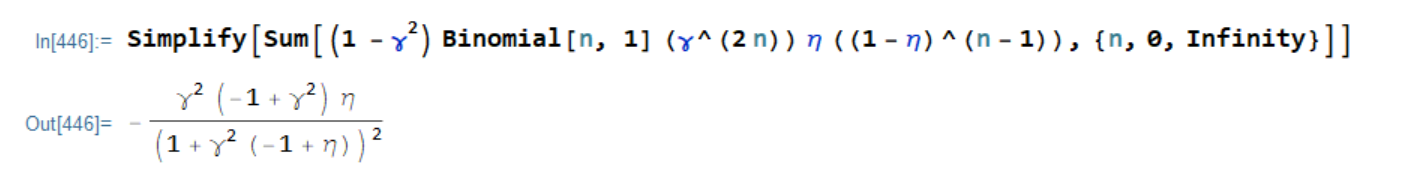
\includegraphics{chapter_05/figs_05/simplify_ppnr.PNG}}

  {\color{darkred} 4 pts for \(p_{PNR}\left(\gamma, \eta\right)\)}

  {\color{midnightblue} Second, derive the single photon fidelity,
  staring with the density matrix for the signal photon given a PNR
  herald event. Using (15) above for
  \(\langle \psi | \Pi_{\text {PNR}} | \psi \rangle\) in the denominator
  helps simplify it significantly. }

  {\color{midnightblue} 

  \[\begin{aligned}
       \rho_s(\gamma,\eta) &= \frac{\operatorname{Tr}_i[\sum_{n=1}^{\infty} \gamma^{2n}n(1-\eta)^{n-1} \eta|n\rangle\langle n|n_s n_i \rangle \langle n_s n_i |]}
           {\langle \psi | \Pi_{\text {PNR}} | \psi \rangle}\\
           |1_s \rangle \langle 1_s | &= \frac{\cancel{(1 - \gamma^2)}(\gamma ^2 (\eta -1)+1)^2 \cancel{\gamma^2 \eta}}{\cancel{\gamma^2 \eta} \cancel{(1 - \gamma ^2)} }\\
           F_{PNR}(\gamma, \eta) &= \boxed{(\gamma ^2 (\eta -1)+1)^2}
   \end{aligned}\]

  }

  {\color{darkred} 4 pts for \(F_{PNR}(\gamma, \eta)\)}

  {\color{midnightblue} For \(\gamma\) near one, the SPDC is under
  strong pump power and is generating predominantly multi-pair states. A
  vanishing fraction of those states are single photon states that the
  PNR detector is able to distinguish and single-photon. Therefore, the
  PNR detector is signaling the generation of multi-pair states most of
  the time which should be discarded and do not contribute to
  \(p_{PNR}\). For high efficiency \(\eta\), only the vanishing
  single-pair creation rate contributes predominantly to \(p_{PNR}\).}

  {\color{darkred} 4 pts for similar explanation}
\item
  (12 pts) Make a parametric plot for \(0<\gamma<1\) with \(F_{PNR}\) on
  the x-axis and \(p_{PNR}\) on the y-axis. Plot the curve for a few
  different values of idler arm efficiency \(0<\eta<1\). All curves
  should reach the same maximum herald probability. What is it?

  {\color{midnightblue}  \textbf{Answer:} }
  {\color{midnightblue} 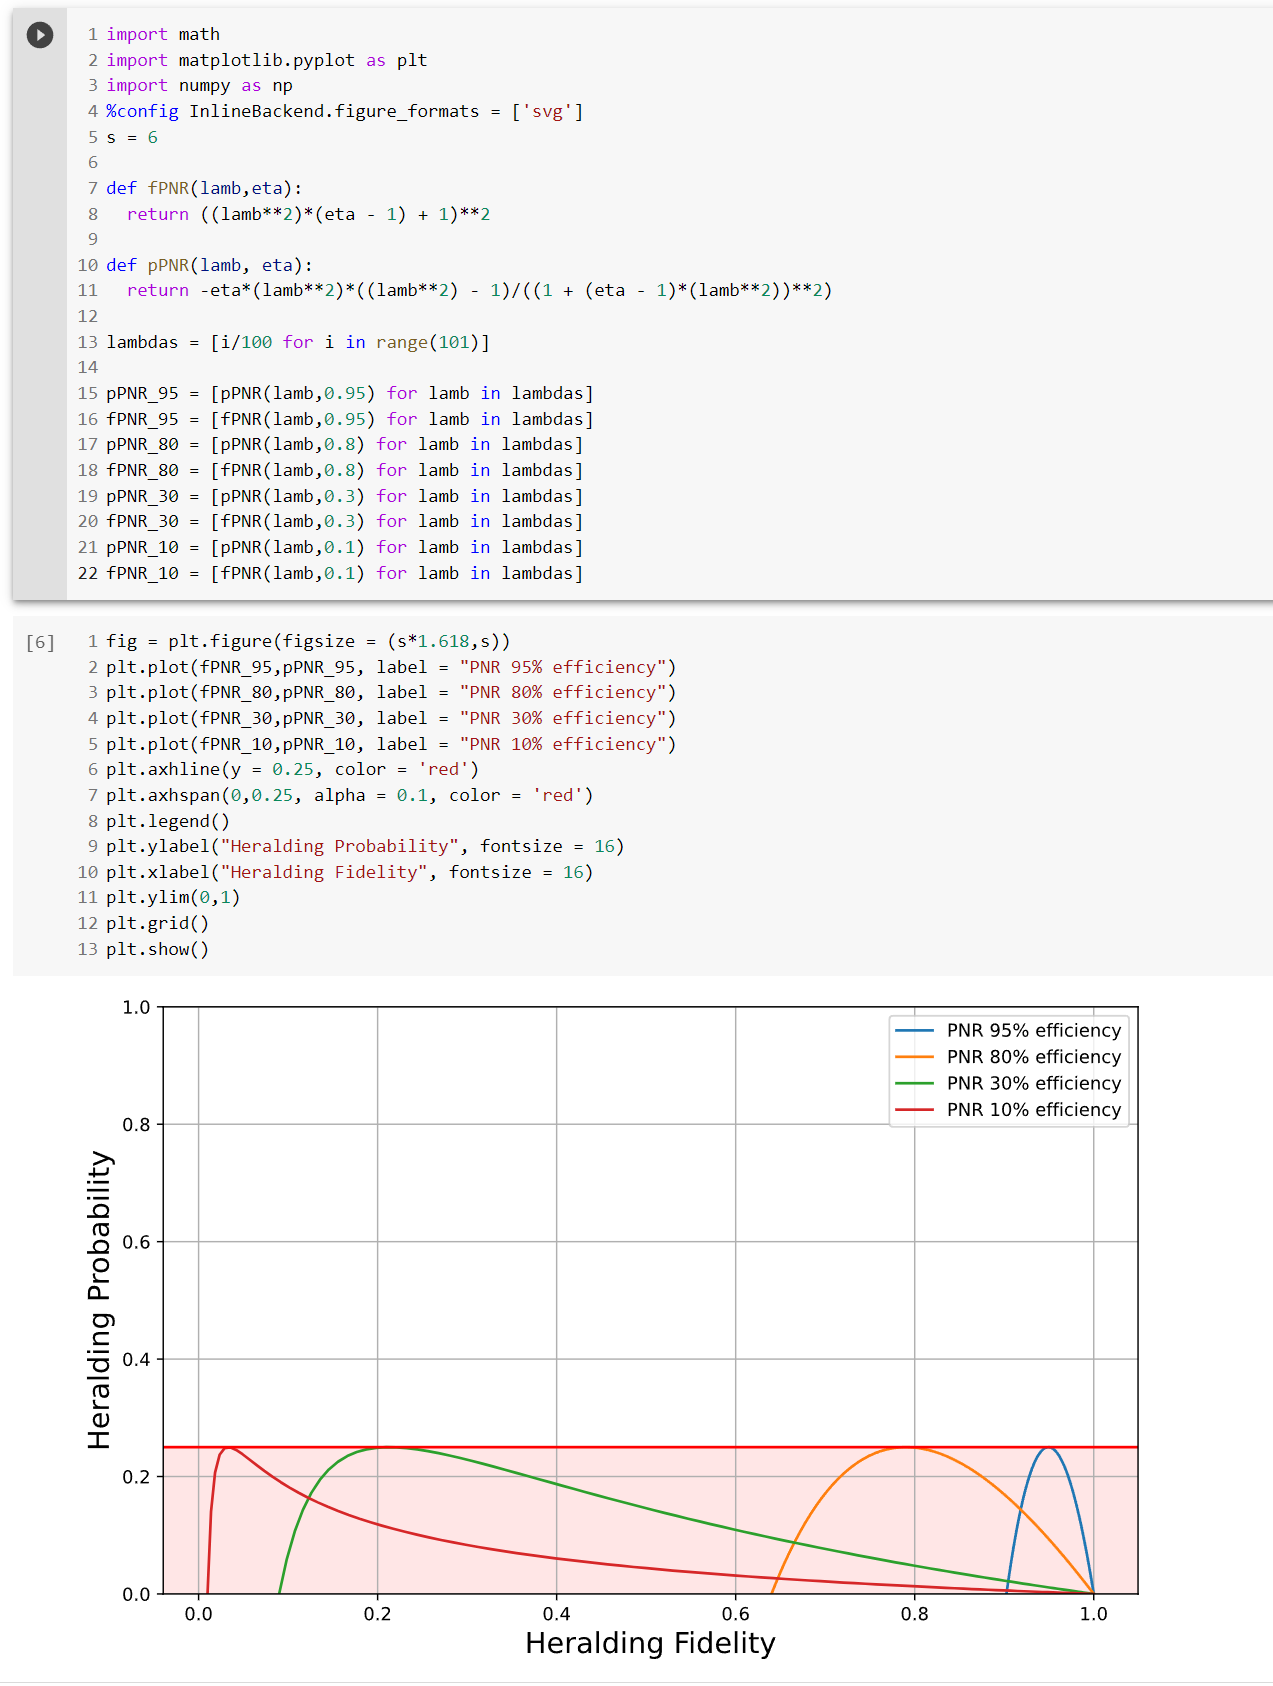
\includegraphics{chapter_05/figs_05/PLT.PNG}}

  {\color{midnightblue}  The the herald probability regardless of idler
  arm efficiency is 25\%. }

  {\color{darkred}  4 points for the 25\% limit; 8 points for a few
  plots at different \(\eta\) }
\item
  (8 pts) Consider again the configuration in Fig.~\ref{fig:hsps} b.
  Find the number of sources using PNR detectors needed to reach 98\%
  single photon herald probability and fidelity with \(\eta = 0.8\).
  Also find the number of sources for \(\eta = 0.95\).

  {\color{midnightblue}  \textbf{Answer:} }
  {\color{midnightblue} 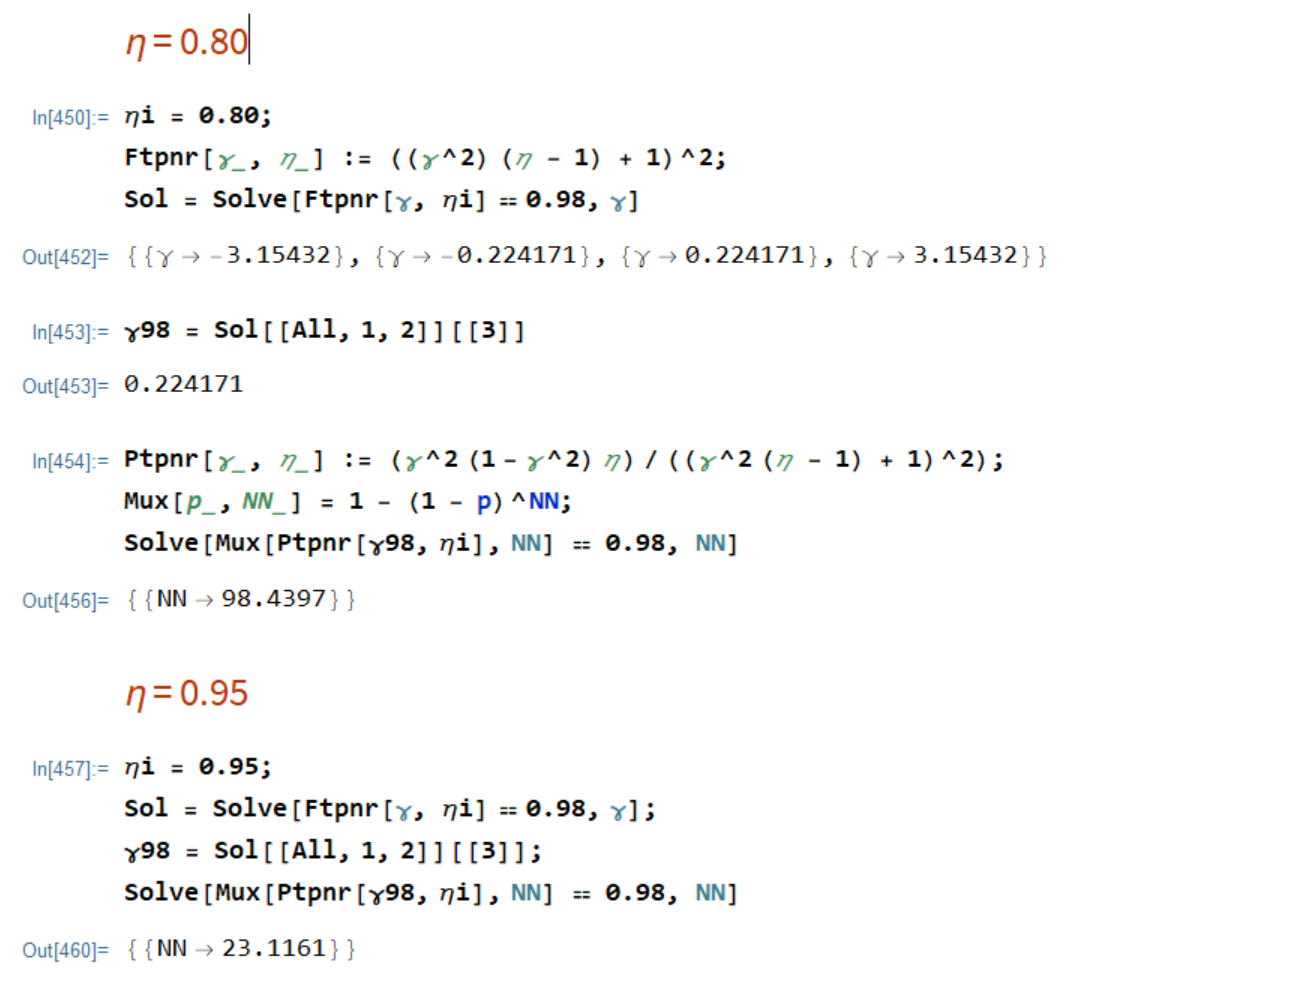
\includegraphics{chapter_05/figs_05/pnrTotalPerf.PNG}}

  {\color{midnightblue} About
  \(\boxed{\text{98 sources are needed for the case with an 80\% heralding}}\),
  }

  {\color{midnightblue} about
  \(\boxed{\text{23 sources are needed with 95\% efficient heralding}}\)}

  {\color{darkred}  4 points for each of the 2 answers. Answers that
  vary from these values by 2-3 sources are acceptable. }
\end{enumerate}

\hypertarget{how-a-sorption-fridge-works}{%
\section{How A Sorption Fridge
Works}\label{how-a-sorption-fridge-works}}

\printbibliography
\end{document}
